\documentclass[11pt,a4paper]{article}
\pdfinfoomitdate=1
\pdftrailerid{}
\usepackage[T1]{fontenc}
\usepackage[utf8]{inputenc}
\usepackage{mathpazo}
\usepackage[scaled=0.92]{helvet}
\renewcommand{\ttdefault}{lmtt}
\usepackage{microtype}
\usepackage[a4paper,margin=2.5cm]{geometry}
\usepackage{amsmath,amssymb}
\usepackage{graphicx}
\usepackage{booktabs}
\usepackage{tabularx}
\usepackage{siunitx}
\sisetup{detect-all, per-mode=symbol}
\usepackage{xcolor}
\usepackage{tikz}
\usetikzlibrary{arrows.meta,positioning,calc}
\usepackage{caption}
\captionsetup{font=small,labelfont=bf,margin=0.5cm}
\usepackage{enumitem}
\setlist{itemsep=2pt,topsep=4pt}
\usepackage{listings}
\lstset{basicstyle=\ttfamily\small,columns=fullflexible,frame=lines,framerule=0.4pt,
        keywordstyle=\color{black}\bfseries,commentstyle=\color{gray},showstringspaces=false,
        xleftmargin=1em,language=Python,aboveskip=8pt,belowskip=8pt}
\usepackage{titlesec}
\titleformat{\section}{\sffamily\Large\bfseries}{\thesection}{0.8em}{}
\titleformat{\subsection}{\sffamily\large\bfseries}{\thesubsection}{0.8em}{}
\titleformat{\subsubsection}{\sffamily\normalsize\bfseries}{\thesubsubsection}{0.8em}{}
\usepackage{fancyhdr}
\pagestyle{fancy}\fancyhf{}
\fancyhead[L]{\sffamily\small Micro-Doppler drone detection with a 60\,GHz radar}
\fancyhead[R]{\sffamily\small A.\,D.\ Canacankatan}
\fancyfoot[C]{\sffamily\small\thepage}
\renewcommand{\headrulewidth}{0.4pt}
\usepackage[hidelinks]{hyperref}
\usepackage{float}

\newcommand{\figw}{\linewidth}
\newcommand{\vmax}{v_{\max}}

\begin{document}

\begin{titlepage}
\setlength{\parindent}{0pt}
\vspace*{1.5cm}
{\sffamily\small TECHNICAL REPORT}\par
\vspace{0.4cm}\hrule\vspace{1.2cm}
{\sffamily\bfseries\huge Detecting a palm-sized drone\\[4pt] by its propeller micro-Doppler\par}
\vspace{0.6cm}
{\sffamily\Large Micro-Doppler measurements and classification with a single-chip 60\,GHz FMCW radar (TI IWR6843AOP), its limits, an independent test, and three short follow-up experiments\par}
\vspace{1.0cm}
{\large Ant Doruk Canacankatan\par}
{\small M.Sc.\ student, Electrical Engineering and Information Technology, Technical University of Munich\par}
\vspace{1.0cm}
\begin{minipage}{0.92\linewidth}
\small\textbf{Summary.}
A spinning propeller moves parts of itself towards and away from a radar at many different speeds at once, so its echo is spread over a wide band of Doppler velocities; a walking person or a fan does not do this in the same way. I used this difference to detect a palm-sized toy quadcopter with a low-cost 60\,GHz radar evaluation board and to tell it apart from a person, a fan and an empty room. I designed a chirp that lets the board stream its full range-Doppler map, wrote the software that records, describes and classifies those maps, and recorded 28 labelled measurements in one room. On recordings the model never saw, 90.7\,\% of one-second windows with a detection were classified correctly (79\,\% of drone windows); counting every window, a drone tethered within about 1.2\,m was recognised in 94\,\% of windows, the one free flight in 10\,\%, and the drone at 1.9\,m not at all. Because these settings were tuned on the same data, I then froze model and code and tested them once on 20 new recordings, partly in a room the system had never seen. In this test no empty room, person or fan was labelled as a drone in any of 1110 frames from ten recordings (not a general false-alarm rate); of the seven drone recordings, five (0.8 to 1.4\,m, two short free flights included) had 98\,\% of their frames labelled as a drone (572 of 583 pooled; 97 to 98\,\% each), one in which the drone fell off its pole had 82\,\%, and the drone at 1.64\,m was missed entirely (0\,\%). The test also exposed three weaknesses: a fan seen with the radar 18\,cm lower was never recognised (100\,\% ``unsure''), a small empty-room margin in one room, and a single-target design that mostly answers ``unsure'' when a person and a fan or drone move at once. The same drone, fan and person were used throughout, so performance in other environments, with other drones and in other geometries is not established. A model-dependent link-budget estimate, not calibrated against a reference reflector, puts the radar cross section of the spinning propellers at the order of 1\,cm$^2$ (0.4 to 1.7\,cm$^2$) and suggests that the range is limited by the simple detection gate rather than by physics. Three follow-ups are reported briefly: seeing a person who stands still (it works once static-clutter removal is switched off, and a held breath is visible), recovering the chest motion from magnitude-only data with the phase retrieval method of my bachelor's thesis (it works in simulation, not yet on real data), and detecting a damaged propeller (in one controlled comparison, cutting half of one blade was associated with a small spectral change; smaller cuts showed none).
\end{minipage}
\vfill
{\small All measurements were planned and carried out by me with my own hardware. The numbers and figures of Sections 6 to 8, Section~\ref{sec:prop} and Appendix~\ref{app:data} are produced from the recorded data by the scripts in Appendix~\ref{app:repro}, with the final version of the code; the few exceptions are listed there.\par}
\end{titlepage}

{\setcounter{tocdepth}{1}\tableofcontents}
\newpage

%=====================================================================
\section{Why this project}
%=====================================================================

Small drones are cheap, fast and hard to see. Optical cameras struggle at night and in fog, and acoustic sensors struggle in noise. Radar works in both, but a palm-sized plastic drone has a tiny radar cross section, often smaller than a bird. What it does have is something birds and people do not: rotors turning at several hundred revolutions per second. Each blade tip moves at tens of metres per second, and as it turns it alternately approaches and recedes from the radar. The resulting echo carries a characteristic \emph{micro-Doppler} signature: energy spread over a wide band of velocities, centred on the (often almost zero) velocity of the body.

The question of this project was simple:
\begin{quote}
\emph{With an off-the-shelf single-chip radar and no special hardware, can I see this signature from a toy drone, and can a small classifier use it to tell the drone apart from a person, a fan and an empty room? Where does it stop working, and why?}
\end{quote}

The second half of the question matters as much as the first. A detection result is only useful if its limits are known, so a large part of this report is about where the method fails: at what distance, for which other objects, and for which reasons.

Section~\ref{sec:physics} derives the physics that the whole project rests on. Section~\ref{sec:hardware} explains the chirp design and why it had to look the way it does. Section~\ref{sec:software} describes the software and the classifier, Section~\ref{sec:measurements} the measurements, and Section~\ref{sec:results} the results. Section~\ref{sec:analysis} analyses the measurements as a radar problem: the scale of the data, the link budget, the drone's radar cross section and what limits the range. Sections~\ref{sec:still}, \ref{sec:pr} and \ref{sec:prop} report three shorter experiments that grew out of the main one. Sections~\ref{sec:limits} and \ref{sec:next} collect the limitations and what I would do next.

%=====================================================================
\section{Physics}\label{sec:physics}
%=====================================================================

\subsection{Measuring distance with a frequency ramp}

The IWR6843 is a frequency-modulated continuous-wave (FMCW) radar. It transmits a \emph{chirp}: a sine wave whose frequency rises linearly with time,
\begin{equation}
f_{\mathrm{tx}}(t) = f_0 + S\,t, \qquad 0 \le t \le T_{\mathrm{ramp}},
\end{equation}
where $f_0 = \SI{60}{GHz}$ is the start frequency and $S$ is the slope in hertz per second. In this project $S = \SI{100}{MHz/\micro s}$.

A target at distance $R$ returns the chirp after the round-trip delay $\tau = 2R/c$. At any instant the received signal therefore has the frequency the transmitter had $\tau$ seconds earlier. The receiver multiplies the received signal with the transmitted one (a mixer) and keeps the difference frequency. This \emph{beat frequency} is
\begin{equation}
f_b = f_{\mathrm{tx}}(t) - f_{\mathrm{tx}}(t-\tau) = S\,\tau = \frac{2 S R}{c}.
\label{eq:beat}
\end{equation}
Distance has become a frequency. With $S = \SI{100}{MHz/\micro s}$, a target at \SI{1}{m} produces $f_b \approx \SI{667}{kHz}$. The beat signal is sampled by the ADC and a Fourier transform over one chirp (the \emph{range FFT}) turns each beat frequency into a peak at the corresponding range.

\paragraph{Range resolution.} The nominal resolution is one FFT bin of the beat frequency, i.e.\ $1/T_{\mathrm{adc}}$ (with the Blackman window that the firmware applies in range, two equal targets must in practice be somewhat further apart to give two separate peaks), where $T_{\mathrm{adc}}$ is the time during which samples are taken. Using~\eqref{eq:beat},
\begin{equation}
\Delta R = \frac{c}{2 S T_{\mathrm{adc}}} = \frac{c}{2B},
\end{equation}
where $B = S\,T_{\mathrm{adc}}$ is the bandwidth swept \emph{while the ADC is sampling}, not the full ramp. Here $T_{\mathrm{adc}} = 64 / \SI{5}{Msps} = \SI{12.8}{\micro s}$, so $B = \SI{1.28}{GHz}$ and $\Delta R = \SI{11.7}{cm}$.

\paragraph{Maximum range.} The ADC samples complex (I/Q) data at $f_s = \SI{5}{Msps}$, so the largest beat frequency it can represent is $f_s$, and
\begin{equation}
R_{\max} = \frac{f_s\,c}{2S} = \SI{7.5}{m}.
\end{equation}
This is the nominal span of the range FFT. TI specifies the usable IF band of this complex sampling mode as about 90\,\% of $f_s$, so in practice the range is limited to about \SI{6.7}{m}; nothing in this project comes close to either value.

\subsection{Measuring velocity from one chirp to the next}

The beat signal also has a phase. For a target at range $R$ the phase of the beat signal is
\begin{equation}
\varphi = \frac{4\pi R}{\lambda},
\label{eq:phase}
\end{equation}
because the wave travels $2R$ and every wavelength $\lambda$ of path adds $2\pi$. At \SI{61.2}{GHz} (the centre of the sampled sweep) $\lambda = \SI{4.90}{mm}$. If the target moves by only $\lambda/2 = \SI{2.45}{mm}$, the phase goes through a full turn. This extreme sensitivity is what makes millimetre-wave radar good at seeing small motion, and it will matter again in Sections~\ref{sec:still} and~\ref{sec:pr}.

The radar transmits $N$ chirps in a row, spaced by $T_c$. A target moving with radial velocity $v$ changes its range by $v T_c$ between chirps, so by~\eqref{eq:phase} its phase advances by
\begin{equation}
\Delta\varphi = \frac{4\pi v T_c}{\lambda}
\end{equation}
from one chirp to the next. A second Fourier transform, this time across the $N$ chirps for each range bin (the \emph{Doppler FFT}), turns this steady phase rotation into a peak at the Doppler frequency
\begin{equation}
f_D = \frac{\Delta\varphi}{2\pi T_c} = \frac{2v}{\lambda}.
\end{equation}

\paragraph{Unambiguous velocity.} A phase step can only be measured modulo $2\pi$. Steps between $-\pi$ and $\pi$ are unambiguous, which limits the speed to
\begin{equation}
|v| < \vmax = \frac{\lambda}{4 T_c}.
\end{equation}
Faster targets \emph{alias}: their energy appears at a wrong velocity, wrapped around from the other end of the axis. With $T_c = \SI{34}{\micro s}$, $\vmax = \SI{36}{m/s}$. This will turn out to be too small for the blade tips of the drone (Section~\ref{sec:microdoppler}).

\paragraph{Velocity resolution.} The Doppler FFT over $N$ chirps has bins of width $1/(N T_c)$ in frequency, i.e.
\begin{equation}
\Delta v = \frac{\lambda}{2 N T_c}.
\end{equation}
With $N = 128$ this is \SI{230}{Hz}, or \SI{0.56}{m/s}.

\subsection{The range-Doppler map, static clutter and the radar equation}

Arranging the result of the two FFTs as a matrix gives the \emph{range-Doppler map}: one row per range bin, one column per velocity bin, and in each cell the echo power at that range moving at that speed. The board combines the four receive antennas and sends this map as a $64 \times 128$ table of 16-bit numbers every frame. All classification in this project works on these maps.

\paragraph{Static clutter removal.} Walls, the table and the radar's own leakage from transmitter to receiver produce strong echoes at zero velocity. The firmware can subtract, for every range bin and antenna, the mean over the $N$ chirps of a frame before the Doppler FFT. Anything that does not change during the \SI{4.35}{ms} of a frame is removed. This makes moving targets stand out, but it also removes things we might want, such as a person who stands still (Section~\ref{sec:still}).

\paragraph{Why small and far is hard.} The received power falls with the fourth power of distance \cite{richards},
\begin{equation}
P_r = \frac{P_t\,G_t G_r\,\lambda^2\,\sigma}{(4\pi)^3 R^4},
\end{equation}
because the wave spreads on the way out and again on the way back. Doubling the distance costs \SI{12}{dB}. The spinning propellers that this project relies on turn out to have a radar cross section $\sigma$ of only about \SI{1}{cm^2} (Section~\ref{sec:rcs}), and the transmit power is of the order of ten milliwatts, so the usable range is short. Together with the simple detection gate, this sets the range limit of the project (Sections~\ref{sec:range} and~\ref{sec:det}).

\subsection{The micro-Doppler of a spinning blade}\label{sec:microdoppler}

Consider one point on a propeller blade at radius $\rho$ from the rotor axis, rotating with angular speed $\Omega = 2\pi f_r$, where $f_r$ is the rotation rate in revolutions per second. Its velocity has magnitude $\rho\Omega$ and turns with the blade. If the plane of rotation makes an angle $\beta$ with the line of sight, the component of that velocity towards the radar is
\begin{equation}
v_\rho(t) = \rho\,\Omega\,\cos\beta\,\sin(\Omega t + \phi_0),
\end{equation}
and its instantaneous Doppler frequency is
\begin{equation}
f_D(t) = \frac{2\rho\Omega\cos\beta}{\lambda}\,\sin(\Omega t + \phi_0).
\label{eq:md}
\end{equation}
This is the micro-Doppler of a rotating point \cite{chen}: a sinusoid in the time-frequency plane whose amplitude grows with radius. A whole blade is a line of such points from the hub to the tip at radius $L$. At any instant it covers every velocity between zero and the tip velocity $v_{\mathrm{tip}} = L\Omega\cos\beta\sin(\Omega t+\phi_0)$.

\paragraph{What the radar sees in one frame.} The 128 chirps of one frame last $N T_c = \SI{4.35}{ms}$ (the coherent dwell; frames repeat every \SI{250}{ms}). A small coreless motor with a propeller turns at roughly 300 to 500 revolutions per second, i.e.\ two or so revolutions per dwell. During one frame every blade therefore sweeps through all angles, so points at all radii and all blade angles contribute to the same frame, at velocities between $-v_{\mathrm{tip}}$ and $+v_{\mathrm{tip}}$. Because the motion is periodic, this energy is in principle concentrated in lines (see the blade flashes below); how evenly it appears spread depends on the geometry, the scattering and the observation time. In the measurements it appears as a broad ``skirt'' around the body velocity (Section~\ref{sec:results}), and this skirt is the feature the whole project is built on.

\paragraph{Tip speed and aliasing.} For a blade of about \SI{2}{cm} at 400 revolutions per second, $v_{\mathrm{tip}} = 2\pi \cdot 400 \cdot 0.02 \approx \SI{50}{m/s}$, larger than $\vmax = \SI{36}{m/s}$. When the rotor is seen nearly edge-on, as here (horizontal rotors, radar at the same height; $|\cos\beta| > 0.72$, i.e.\ within about $44^\circ$ of edge-on), the outer part of the blade would then exceed $\vmax$, alias and be folded back onto the velocity axis. The rotation rate was not measured, so this is an estimate: below about 290 revolutions per second the tips would stay just under the limit and still sweep almost the whole axis. In the closest measurement (\SI{0.6}{m}) the drone has energy in almost every Doppler bin (\emph{occupancy} 0.50, Section~\ref{sec:features}); this is consistent with aliasing but does not prove it. Further away the occupancy is much lower (0.02 to 0.13), because most of the spread lies below the noise floor. It is a nuisance for estimating the rotation rate, but it makes the drone easy to recognise.

\paragraph{Blade flashes and spectral lines.} When a blade is perpendicular to the line of sight its whole length reflects in phase and the echo flashes. With an even number $N_b$ of identical blades, as on a two-blade toy propeller, the flashes repeat $N_b f_r$ times per second (with an odd number, $2N_b f_r$). A periodic signal in time has a line spectrum, so the Doppler spectrum of a perfect rotor consists of lines spaced $N_b f_r$ apart (often called helicopter rotor modulation lines). For a two-blade toy propeller at 400\,rev/s the spacing would be about \SI{800}{Hz}, three to four of our \SI{230}{Hz} Doppler bins. In practice four rotors at slightly different speeds and the aliasing above smear these lines together, and I could not resolve them reliably (Section~\ref{sec:features}). An unbalanced or damaged blade breaks the symmetry between the blades and adds lines at multiples of $f_r$ itself; this is the idea behind Section~\ref{sec:prop}.

\subsection{What a person and a fan look like}

A walking person moves the torso at about 1 to \SI{1.5}{m/s} and the arms and legs at up to a few metres per second. Almost all of the energy stays within $|v| < \SI{5}{m/s}$, and the strongest part is the torso. A stand fan has long blades turning slowly (around 1000 revolutions per minute) and, seen face-on, its blades move mostly across the line of sight, so $\cos\beta$ in~\eqref{eq:md} is small. Its spectrum is therefore narrower than the drone's and widens with fan speed, which is exactly what the measurements show (Figure~\ref{fig:fanspeed}). The empty room, after clutter removal, is noise plus a few fixed artefacts of the board.

%=====================================================================
\section{Hardware and chirp design}\label{sec:hardware}
%=====================================================================

\subsection{The board}

The radar is a Texas Instruments IWR6843AOPEVM: a single-chip 60 to 64\,GHz FMCW radar with three transmit and four receive antennas built into the chip package, on a small evaluation board with a USB connection. It runs TI's ``out-of-box'' demo firmware from the mmWave SDK 3.x, which I did not modify. The firmware accepts a text configuration on one serial port (\SI{115200}{baud}) and streams binary results on a second port (\SI{921600}{baud}). This firmware sends no raw ADC data over the serial link (raw samples would need a separate capture board, Section~\ref{sec:next}); everything in this report is computed from what it sends: the range-Doppler map, the range profile and a point list.

\subsection{Designing the chirp}

The default configurations shipped with the demo use all three transmitters for angle estimation and do not send the range-Doppler map at a useful rate. For micro-Doppler the priorities are different: the full map every frame, a high unambiguous velocity and enough Doppler bins. The binding constraint turned out to be the serial link. One map of $64 \times 128$ cells at two bytes each is \SI{16}{KB}; at \SI{921600}{baud} with ten bits on the wire per byte this takes
\[
\frac{16384 \times 10}{921600}\,\mathrm{s} = \SI{178}{ms}.
\]
The frame period must be longer than this, so I chose \SI{250}{ms}, i.e.\ four frames per second. Within that budget the other parameters were chosen as follows (Table~\ref{tab:chirp}):
\begin{itemize}
\item \textbf{One transmitter.} With time-division multiplexing of three transmitters the chirp period seen by each one triples and $\vmax$ drops to \SI{12}{m/s}. With one transmitter, $T_c = \SI{34}{\micro s}$ and $\vmax = \SI{36}{m/s}$.
\item \textbf{64 samples at 5\,Msps, slope 100\,MHz/\textmu s.} This gives 64 range bins of \SI{11.7}{cm} up to \SI{7.5}{m}: fine enough to separate a drone from a person behind it, and only 64 rows so that the map fits the link.
\item \textbf{128 chirps.} The most Doppler bins that fit; each is \SI{0.56}{m/s} wide.
\end{itemize}
Two practical lessons: the AOP firmware rejects the \texttt{bpmCfg} command that appears in many example files, and the board is sensitive to the USB cable moving; the software now reports a lost connection clearly and keeps what it had recorded.

\begin{table}[h]
\centering\small
\caption{Chirp configuration \texttt{md\_1tx.cfg} and the quantities derived from it. The software derives the same numbers from the configuration file, so every axis in every figure comes from the chirp that was actually sent.}
\label{tab:chirp}
\begin{tabular}{@{}llll@{}}
\toprule
Set in the configuration & Value & Derived & Value \\
\midrule
Start frequency & \SI{60}{GHz} & Wavelength (sampled-sweep centre) & \SI{4.90}{mm}\\
Slope & \SI{100}{MHz/\micro s} & Sampled bandwidth $B$ & \SI{1.28}{GHz}\\
ADC samples, rate & 64, \SI{5}{Msps} & Range resolution $\Delta R$ & \SI{11.7}{cm}\\
Idle + ramp time & \SI{10}{} + \SI{24}{\micro s} & Maximum range (nominal) & \SI{7.5}{m}\\
Transmitters, receivers & 1, 4 & Chirp period $T_c$ & \SI{34}{\micro s}\\
Chirps per frame & 128 & Max.\ unambiguous velocity & \SI{\pm 36}{m/s}\\
Frame period & \SI{250}{ms} & Doppler bin & \SI{230}{Hz} = \SI{0.56}{m/s}\\
Static clutter removal & on & Map size, transfer time & \SI{16}{KB}, \SI{178}{ms}\\
\bottomrule
\end{tabular}
\end{table}

%=====================================================================
\section{Software}\label{sec:software}
%=====================================================================

The software is a small Python package (about 1600 lines) plus about 450 lines of command-line scripts. Figure~\ref{fig:chain} shows the path from the antenna to a label on the screen.

\begin{figure}[h]
\centering
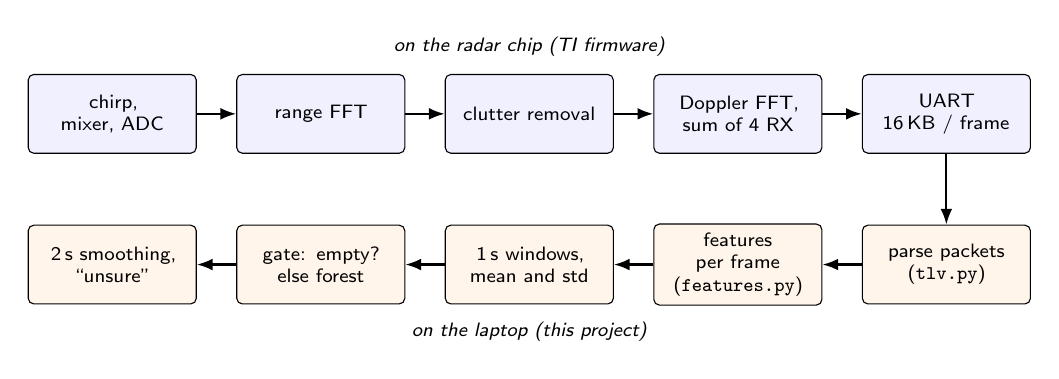
\begin{tikzpicture}[node distance=4mm and 5mm, every node/.style={font=\sffamily\scriptsize},
  box/.style={draw, rounded corners=2pt, align=center, minimum height=10mm, text width=19mm, fill=gray!6},
  chip/.style={box, fill=blue!6}, pc/.style={box, fill=orange!8}, ar/.style={-{Latex[length=2mm]}, thick}]
\node[chip] (a) {chirp,\\ mixer, ADC};
\node[chip, right=of a] (b) {range FFT};
\node[chip, right=of b] (c) {clutter removal};
\node[chip, right=of c] (d) {Doppler FFT, sum of 4 RX};
\node[chip, right=of d] (e) {UART\\ 16\,KB / frame};
\node[pc, below=9mm of e] (f) {parse packets\\ (\texttt{tlv.py})};
\node[pc, left=of f] (g) {features per frame\\ (\texttt{features.py})};
\node[pc, left=of g] (h) {1\,s windows, mean and std};
\node[pc, left=of h] (i) {gate: empty?\\ else forest};
\node[pc, left=of i] (j) {2\,s smoothing, ``unsure''};
\draw[ar] (a)--(b); \draw[ar] (b)--(c); \draw[ar] (c)--(d); \draw[ar] (d)--(e);
\draw[ar] (e)--(f); \draw[ar] (f)--(g); \draw[ar] (g)--(h); \draw[ar] (h)--(i); \draw[ar] (i)--(j);
\node[above=1mm of c, font=\sffamily\scriptsize\itshape] {on the radar chip (TI firmware)};
\node[below=1mm of h, font=\sffamily\scriptsize\itshape] {on the laptop (this project)};
\end{tikzpicture}
\caption{Processing chain. The upper row runs in TI's firmware on the radar; the lower row is the software written for this project.}
\label{fig:chain}
\end{figure}

\subsection{Talking to the board}

\texttt{radar.py} finds the two serial ports by sending the command \texttt{version} to each and seeing which one answers, sends the configuration line by line and stops with a readable message if the board rejects a line. A background thread reads the data port and hands the bytes to the parser.

\texttt{tlv.py} parses the binary stream. Every packet starts with a 40-byte header, beginning with a fixed 8-byte magic word, that gives the frame number and the number of type-length-value (TLV) blocks that follow. The range-Doppler map arrives as TLV type 5: 8192 unsigned 16-bit values, each the base-2 logarithm of a magnitude in Q9 fixed point, so one unit equals $20\log_{10}2/512 \approx \SI{0.0118}{dB}$ according to answers in TI's support forum (the SDK documentation \cite{ti-uart} gives the TLV type and the 16-bit format but not this scale). Section~\ref{sec:scale} shows that the true scale is about twice this. \emph{All dB values in this report are given in these ``map units'' unless they are explicitly called true dB}; differences in true dB are about twice as large. The classifier was trained and tested on the same scale, so its accuracy is unaffected; but quantities computed from the map are not physical powers (see the note after the feature list). Zero velocity is in the first column; the parser shifts it to the centre. The parser is written so that it never trusts a length field without checking it against the bytes it has, which matters because a moving cable can cut a packet in half.

\subsection{Recording and simulating}

\texttt{record.py} saves every measurement twice: the raw byte stream as it arrived, and a compressed NumPy file with the decoded maps, timestamps, the configuration text and a label, distance and free-text note. The raw stream can be replayed through the live view as if the board were connected (the raw files are not published); the published \texttt{.npz} recordings are replayed through the classifier by \texttt{eval\_test.py}.

\texttt{sim.py} is a point-scatterer simulator of the same chirp. It models the four receive antennas of the AOP package and targets made of points: a quadcopter with four two-blade rotors, a walking person with swinging limbs, a fan, and static reflectors. It generates the beat signal sample by sample and runs it through a processing chain modelled on the firmware's; the way it combines the antennas is an approximation (Section~\ref{sec:sim}). It let me write and test all of the software before the drone arrived, and later served as a reference to compare the measurements against (Section~\ref{sec:sim}).

\subsection{Describing one map with a few numbers}\label{sec:features}

Rather than feeding raw maps to a large network, which with a few thousand frames from one room would mostly learn the room, I describe each map with nine numbers that each have a physical meaning. Let $M(r,k)$ be the map in dB, $r$ the range bin and $k$ the Doppler bin with $k=0$ at zero velocity.
\begin{enumerate}
\item \textbf{Floor} $F = \operatorname{median}_{r,k} M(r,k)$. Most cells contain only noise, so the median is a robust noise estimate.
\item \textbf{Target range} $r^\ast$: the range bin, beyond \SI{0.45}{m}, with the most linear power outside the zero-velocity bins $|k| \le 1$. The cut at \SI{0.45}{m} excludes fixed artefacts of the board described in Section~\ref{sec:wrong}.
\item \textbf{Spectrum} $s(k) = \max_{|r-r^\ast| \le 1} M(r,k) - F$, the Doppler spectrum at the target, in dB above the floor.
\end{enumerate}
From $s(k)$ and the map, over the moving bins $|k| > 1$:
\begin{itemize}
\item \texttt{snr\_db}: $\max_k s(k)$, the strength of the target.
\item \texttt{occupancy}: the share of moving bins with $s(k) > \SI{6}{dB}$. A spinning rotor, whose energy is spread and aliased over the whole axis, gives about 0.5 at short range; a person gives about 0.02.
\item \texttt{skirt\_db}: $10\log_{10}$ of the mean linear power for $10 < |v| < \SI{25}{m/s}$. Only fast-moving parts reach this band; in these data mainly the propellers (the fan shows a few isolated peaks there, Figure~\ref{fig:spectra}).
\item \texttt{high\_v\_frac}: the share of the moving power at $|v| > \SI{10}{m/s}$.
\item \texttt{flatness}: geometric over arithmetic mean of the linear spectrum; 1 for white noise, near 0 for a single line.
\item \texttt{v\_centroid}: the power-weighted mean speed $|v|$.
\item \texttt{range\_extent}: the number of range bins (beyond \SI{0.45}{m}) containing a moving cell \SI{15}{dB} above the floor. A person is extended in range, a drone is not.
\item \texttt{period\_score} and \texttt{line\_spacing\_hz}: height and lag of the largest peak in the autocorrelation of the detrended spectrum. They were meant to catch the blade-flash lines of Section~\ref{sec:microdoppler}. In practice they are weak features, as expected from the smearing discussed there.
\end{itemize}
Here ``linear power'' means $10^{m/10}$ of a map value $m$. Since one map unit is about two true dB (Section~\ref{sec:scale}), this is closer to the echo amplitude than to its power, so the features are empirical functions of the map rather than physically power-weighted quantities. They are used identically in training and test.

One boundary defect was found after the test: when $r^\ast$ is the first allowed bin (\SI{0.47}{m}), the spectrum $s(k)$ also takes its lower neighbour at \SI{0.35}{m}, inside the excluded artefact zone. This happened in 91 of 5084 frames (1.8\,\%), mostly in the free flight, the swinging drone and the hand in front of the radar. It is part of the frozen pipeline and was left unchanged; a corrected version would need a new evaluation. Two more properties of the frozen code were found later and left unchanged for the same reason. Windows are formed from consecutive stored frames, also across the rare gaps where the board dropped a frame: 13 of the 988 detected windows span such a gap, and leaving them out of the cross-validation gives 881 of 975 (90.4\,\%) instead of 896 of 988 (90.7\,\%). And the detrending in the line feature pads the spectrum with zeros at its ends, so \texttt{period\_score} changes slightly when the whole map is shifted by a constant; it is one of the two weakest features (Section~\ref{sec:classif}). Finally, a window whose mean is exactly at the gate is kept for training but treated as empty in the live classifier; no window in the recordings comes within \SI{0.001}{dB} of the gate, so this affects no result.

The skirt feature is computed as
\begin{lstlisting}
s     = spec - floor                 # spectrum at the target, dB above the floor
band  = (np.abs(v) > 10) & (np.abs(v) < 25)
skirt = 10 * np.log10(np.mean(10 ** (s[band] / 10)))
\end{lstlisting}
The frame rate is four per second, and a single frame can be misleading (a blade can be in a bad position, a person can pause). Features are therefore aggregated over windows of four frames (one second), stepping by two frames, as their mean and standard deviation: 18 numbers per window.

\subsection{Two stages: is anything there, and what is it?}

My first classifier treated ``empty'' as a fourth class and confused it badly with everything else. The reason is that an empty window has no target, so its features describe noise and are almost random. The final design separates the two questions:
\begin{enumerate}
\item \textbf{Detection gate.} A window is \emph{empty} if the mean \texttt{snr\_db} of its four frames is at most \SI{8}{dB}. In five empty-room recordings the largest window mean was \SI{7.2}{dB}, so the gate has a margin of \SI{0.8}{dB}.
\item \textbf{Classification.} Windows above the gate go to a random forest (300 trees, at least two samples per leaf, classes weighted inversely to their frequency) that chooses between \emph{drone}, \emph{human} and \emph{fan}.
\end{enumerate}
A random forest was chosen because it needs no feature scaling, copes with features of very different usefulness, and reports which features it relied on. With about a thousand windows a deep network would not have been justified.

\subsection{Evaluation grouped by recording}

Neighbouring windows of the same recording are nearly identical. If windows were shuffled randomly into training and test sets, the model would be tested on near-copies of what it was trained on and the accuracy would be inflated. All evaluation in this report is therefore \emph{grouped by recording}: every recording is either entirely in the training set or entirely in the test set (five-fold grouped cross-validation, and leave-one-recording-out for the live replay).

This protects against near-duplicate windows, but not against everything. The features, the \SI{0.45}{m} range cut, the detection gate, the guard bins and the confidence thresholds were all chosen while looking at these same recordings, and some were changed after seeing which recordings failed. The cross-validated numbers in this report are therefore likely to be optimistic. To check this, every setting was frozen and the system was tested once on new recordings in the same room and in a second room (Section~\ref{sec:test}). The one-second windows also overlap by half, so the 988 windows are far from 988 independent trials; the uncertainty is better judged from the variation between recordings and folds (Section~\ref{sec:classif}).

\subsection{The live view}

\texttt{live.py} shows the map, the Doppler spectrum at the target and the label, updated every frame. A first live test (Section~\ref{sec:live}) showed short false ``drone'' labels whenever a hand or arm moved close to the radar. Three rules were added:
\begin{itemize}
\item the class probabilities of the last eight frames (two seconds) are averaged before choosing a label;
\item if the averaged winner is below 60\,\% probability, the label is \emph{unsure} instead of a guess;
\item \emph{drone} needs 70\,\%, because a false drone alarm costs more than a late one.
\end{itemize}

%=====================================================================
\section{Measurements}\label{sec:measurements}
%=====================================================================

All development recordings (training, cross-validation and the follow-ups) were made in one furnished room; seven recordings of the independent test (Section~\ref{sec:test}) were made in a second room. The radar stood on the desk, raised on a small stand. The drone was a palm-sized toy quadcopter with four two-blade propellers inside a thin plastic guard (Figure~\ref{fig:photos}).

\begin{figure}[h]
\centering
\begin{minipage}[b]{0.66\linewidth}\centering
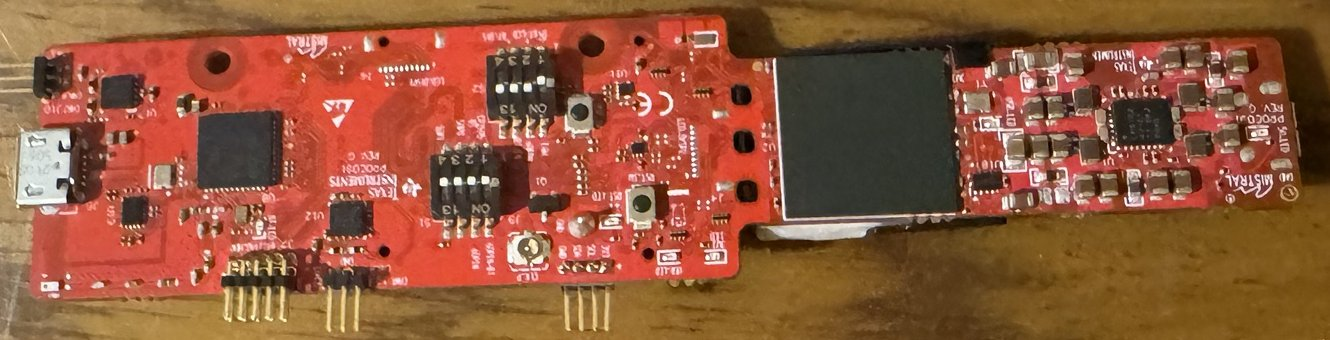
\includegraphics[width=\linewidth]{figs/photo_board.jpg}\\[2pt]
{\small (a) the radar evaluation board, USB connector on the left}
\end{minipage}\hfill
\begin{minipage}[b]{0.3\linewidth}\centering
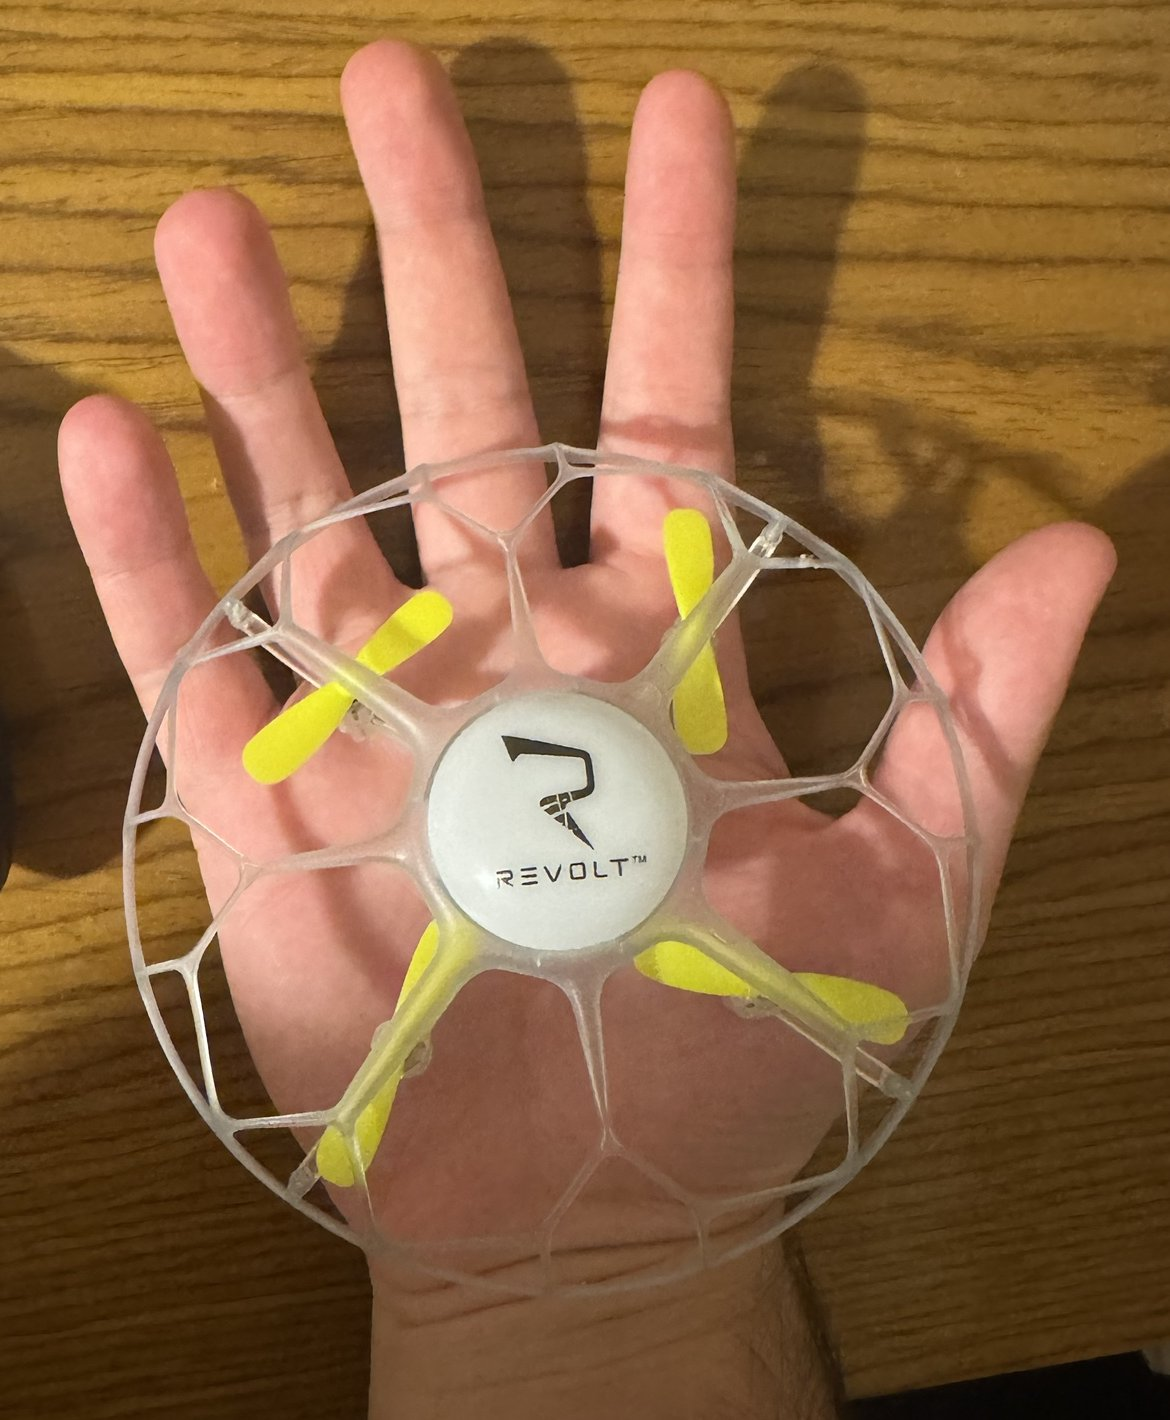
\includegraphics[width=\linewidth]{figs/photo_drone.jpg}\\[2pt]
{\small (b) the drone, for scale}
\end{minipage}
\caption{The hardware: the TI IWR6843AOPEVM radar board and the toy quadcopter.}
\label{fig:photos}
\end{figure}
 Because it cannot hold position on its own, most drone recordings were made with it tied to the end of a long pole that was itself taped to fixed furniture (no hand on it), so that it ran at full throttle at the height of the pole without being able to fly away, at a fixed distance from the radar, with me standing well behind it or behind the radar. For the propeller experiment it was taped to a short stick instead. Distances were set with a tape measure but are approximate for the tethered drone; the range reported by the radar is used in the analysis. As a check, a metal pot placed at \SI{0.70}{m} by tape was reported at \SI{0.68}{m}.

The labelled data set used for classification contains 28 recordings of about 19 to 40 seconds (Table~\ref{tab:data} in Appendix~\ref{app:data}):
\begin{itemize}
\item \textbf{empty room}, 5 recordings at different times, with me outside the room for the last two;
\item \textbf{fan}, 8 recordings: a stand fan at \SI{2}{m}, \SI{1}{m} and \SI{0.8}{m} (side-on), at speed settings 1 to 3, one repeated;
\item \textbf{human}, 9 recordings: walking towards and away at about \SI{2.5}{m}, walking close at \SI{0.7}{m}, waving arms at \SI{2}{m} and \SI{0.7}{m}, moving a hand at \SI{0.5}{m}, standing almost still and sitting with small hand movements at \SI{1.2}{m};
\item \textbf{drone}, 6 recordings: one free flight (it went out of control), and tethered at about 0.5, 0.7 (straight and to the left), 1.0 and \SI{1.7}{m}.
\end{itemize}
Further recordings for the follow-up experiments (breathing, phase retrieval, propeller damage) are listed with their sections.

%=====================================================================
\section{Results}\label{sec:results}
%=====================================================================

\subsection{What the four classes look like}

Figure~\ref{fig:rd} shows range-Doppler maps averaged over a whole recording for one example of each class. The empty room is dark apart from a few fixed spots below \SI{0.4}{m}. The person waving their arms is a compact blob at their range: strong, but confined to a few metres per second, with the arms adding a little width around the torso. A walking person looks similar but is smeared along range in a recording-long average, because the range changes. The fan is a broader blob, with fainter copies at larger range that are multipath reflections (the echo bouncing off the fan and then a wall). The drone is unmistakable: a horizontal band at its range that covers the entire velocity axis.

\begin{figure}[t]
\centering
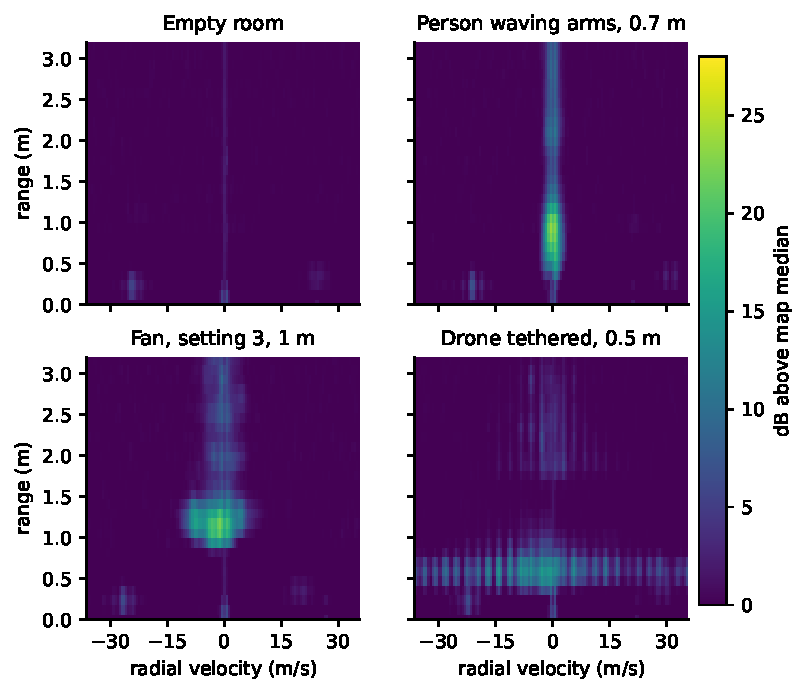
\includegraphics[width=0.86\linewidth]{figs/rd_maps.pdf}
\caption{Range-Doppler maps, power-averaged over each recording and shown relative to the map median (map units). Static objects are removed by the firmware. The drone's energy spans almost the whole velocity axis: its blade tips move at speeds close to or above the \SI{36}{m/s} limit (Section~\ref{sec:physics}).}
\label{fig:rd}
\end{figure}

\begin{figure}[t]
\centering
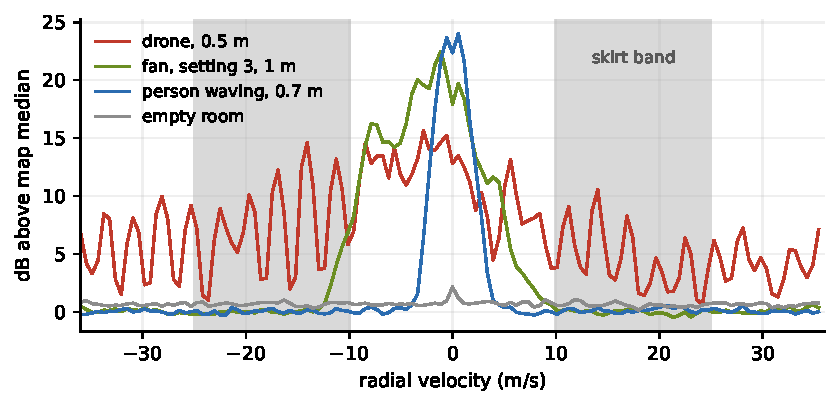
\includegraphics[width=0.9\linewidth]{figs/spectra.pdf}
\caption{Doppler spectrum at the target range, averaged over each recording. Only the drone has energy well above the floor across the grey ``skirt'' band at 10 to \SI{25}{m/s}; the fan has a few isolated peaks there.}
\label{fig:spectra}
\end{figure}

Figure~\ref{fig:spectra} shows the same thing as spectra at the target range. In the skirt band the drone at \SI{0.5}{m} sits about \SI{7}{dB} above the floor, while the fan, the person and the empty room are within about \SI{1}{dB} of it.

\begin{figure}[t]
\centering
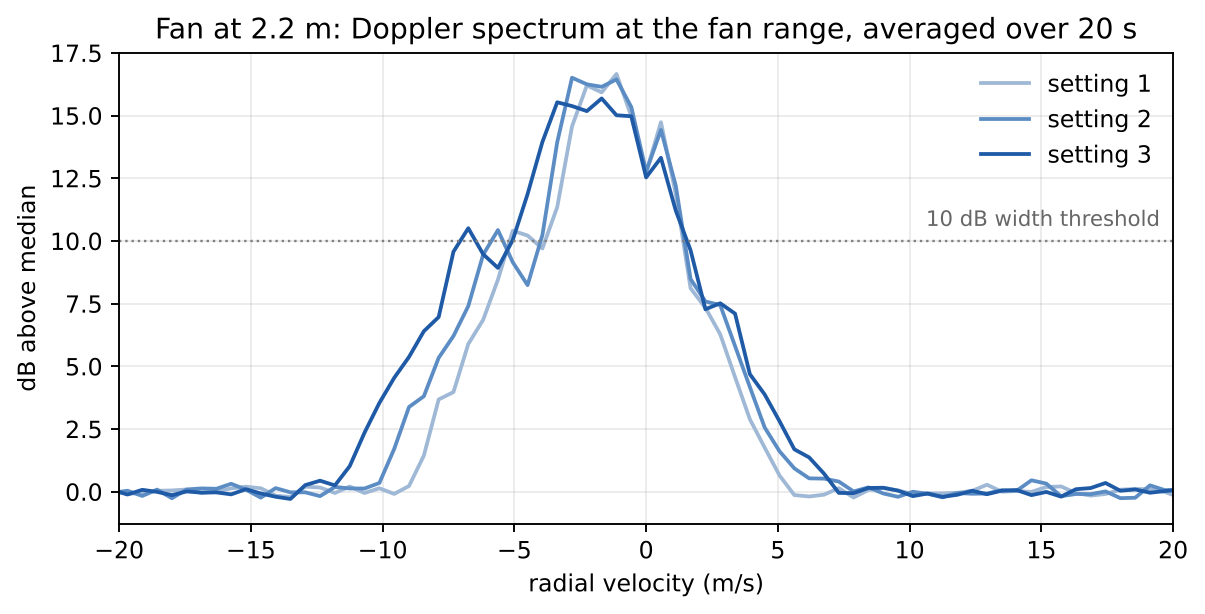
\includegraphics[width=0.78\linewidth]{figs/fig_fan_spectra.png}
\caption{Fan at a nominal \SI{2}{m} (\SI{2.2}{m} measured by the radar): the spectrum widens with fan speed, as expected from the higher blade-tip speed.}
\label{fig:fanspeed}
\end{figure}

The fan behaves as the physics predicts. Measured as the width of the spectrum more than \SI{10}{dB} above the floor, it grows with the speed setting: 6.2, 6.8 and \SI{7.9}{m/s} at \SI{2}{m} for settings 1, 2 and 3 (Figure~\ref{fig:fanspeed}); a repeated setting-3 recording gave the same \SI{7.9}{m/s}. At \SI{1}{m} the widths are 10.1 and \SI{13.5}{m/s} for settings 1 and 3. A fast fan is therefore the closest thing to a drone in this data set, which shows up again in the classification.

\subsection{Is there anything there? The detection gate}

None of the five empty-room recordings produced a single window above the gate. Of the recordings with a target, all fan recordings and all human recordings except one were detected in every window; the exception is the sitting person making only small hand movements at \SI{1.2}{m}, detected in 54\,\% of windows. A still body is removed by clutter removal along with the furniture (Section~\ref{sec:still} returns to this).

\subsection{How far away can the drone be?}\label{sec:range}

In this subsection distances are the ranges measured by the radar, which differ from the approximate tape distances given elsewhere (for example, the drone tethered at a nominal \SI{0.5}{m} is seen at \SI{0.59}{m}, the one at \SI{1}{m} at \SI{1.17}{m}). Figure~\ref{fig:distance} shows the median peak SNR and skirt level of the tethered-drone recordings against this range. At \SI{0.6}{m} the drone is strong (SNR \SI{16.5}{dB}, skirt \SI{7.5}{dB}). At \SI{1.2}{m} it is still detected in every window (SNR \SI{11.4}{dB}), but its skirt has dropped to \SI{2.3}{dB}, close to the range of values that fans and people produce. At \SI{1.9}{m} the median SNR is \SI{6.7}{dB} and no window passes the gate. Nothing between 1.2 and \SI{1.9}{m} was measured, so the maximum range lies somewhere in that interval and is not known more precisely; all of these are tethered-drone measurements. In the development free flight (R11) there is no ground-truth distance: windows whose selected range lay between 0.7 and \SI{1.3}{m} passed the gate in 18 of 20 cases, and further out the selected range itself is unreliable. The two free flights of the independent test (Section~\ref{sec:test}), at about 0.8 to \SI{1.2}{m}, passed it in every window.

The drop from \SI{0.6}{m} to \SI{1.2}{m} is about \SI{5}{dB} in peak SNR in map units. At first this looked too small for the \SI{12}{dB} the $R^{-4}$ law predicts; it led to the finding of Section~\ref{sec:scale} that one map unit is about two true dB, after which the drop is close to the radar equation. The skirt falls faster than the peak. The reason is not established here: a fixed noise floor would, if anything, make a weak band fall more slowly, so the faster drop must come from the echo in that band itself (for example its dependence on the viewing angle of the blade tips). The recording taken \SI{46}{\degree} off the boresight has a weaker skirt than the one at \SI{1.2}{m} although it is closer, consistent with the antenna pattern and with the blades being seen from a different angle.

\begin{figure}[t]
\centering
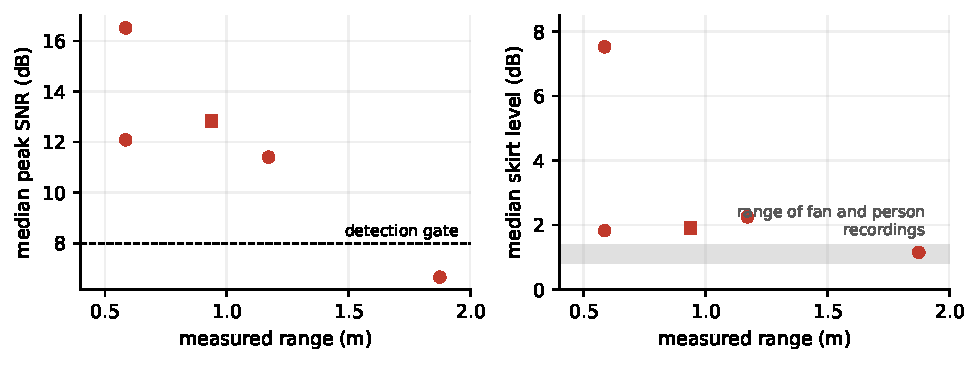
\includegraphics[width=0.92\linewidth]{figs/distance.pdf}
\caption{Tethered drone at different ranges (square: \SI{46}{\degree} off boresight; lower point near \SI{0.6}{m}: the drone moving on its tether, nominal \SI{0.7}{m}). Left: median peak SNR with the detection gate. Right: median skirt level; the grey band is the range of values in the fan and person recordings with more than 90\,\% of windows above the gate (all but R26, whose value lies inside the band).}
\label{fig:distance}
\end{figure}

One more observation from the \SI{1.9}{m} recording: even though no window passed the gate, the target range found in each frame was the same bin in 78\,\% of frames and within one bin in 92\,\%. The drone was there, below the detection gate but not below the noise (Section~\ref{sec:det}). Section~\ref{sec:det} shows what this means for the range limit.

\subsection{Classification}\label{sec:classif}

Over the 22 recordings with windows above the gate (988 one-second windows: 289 drone, 391 human, 308 fan), grouped five-fold cross-validation gives \textbf{90.7\,\%} correct windows, against 33\,\% for guessing. This is the accuracy of the second stage only, i.e.\ of telling drone, person and fan apart \emph{once something has been detected}; it is not a drone detection rate. Figure~\ref{fig:cm} shows the confusion matrix. Per class, 79\,\% of drone windows, 94\,\% of human windows and 98\,\% of fan windows were classified correctly; of the windows labelled drone, 92\,\% were drone.

\paragraph{How uncertain is this?} The five folds gave 94, 99, 65, 99 and 94\,\%: the accuracy depends strongly on which recordings end up in the test set (the 65\,\% fold contains the free flight). Resampling whole recordings with replacement (5000 bootstrap draws) gives a 95\,\% interval of roughly 80 to 98\,\% for the overall accuracy, and 45 to 100\,\% for the drone class alone, which rests on only five recordings with detected windows (the drone at \SI{1.9}{m} has none). These intervals are rough, but they are a fairer summary than the single number.

\begin{figure}[t]
\centering
\begin{minipage}{0.4\linewidth}\centering
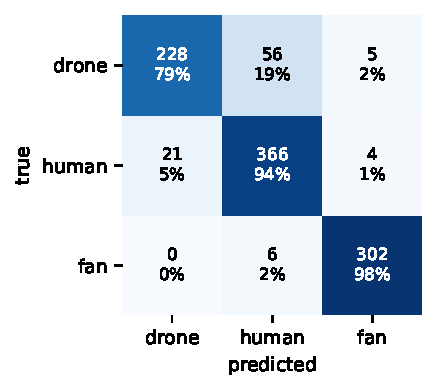
\includegraphics[width=\linewidth]{figs/confusion.pdf}
\end{minipage}\hfill
\begin{minipage}{0.56\linewidth}\centering
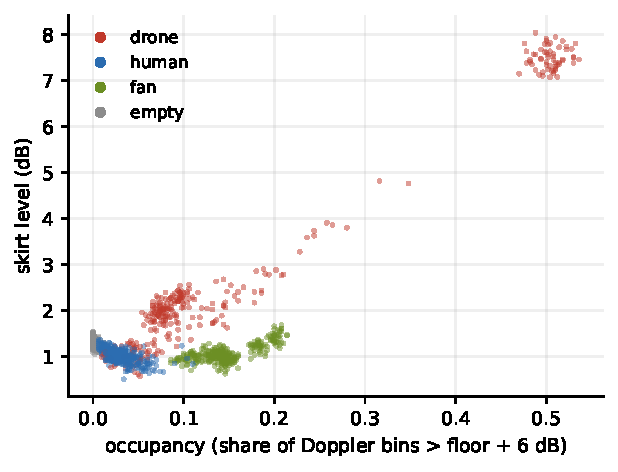
\includegraphics[width=\linewidth]{figs/feature_space.pdf}
\end{minipage}
\caption{Left: confusion matrix of grouped five-fold cross-validation (counts and row percentages). Right: the one-second windows above the detection gate and the empty-room windows, in two of the 18 dimensions (the 84 drone and 18 person windows below the gate are not shown). Drone windows at short range sit far from everything else; the drone cloud near the origin comes from the free-flight and longer-range recordings.}
\label{fig:cm}
\end{figure}

Almost all errors come from a few recordings, and each has a physical explanation:
\begin{itemize}
\item \textbf{The out-of-control flight} (54 windows, 15\,\% correct). The drone tumbled through the room at 0.5 to \SI{1.5}{m}. Most of its windows look like a person: the whole drone moving fast dominates the spectrum, and at the far end of its path the skirt disappears.
\item \textbf{The tethered drone moving around at 0.7\,m} (75\,\% correct), whose moving body adds a person-like component.
\item \textbf{The sitting person with small hand movements} (21 windows above the gate, 48\,\% correct), the weakest human recording.
\item \textbf{A hand moved right in front of the radar} (84\,\%) and \textbf{arm waving at 2\,m} (87\,\%).
\item \textbf{The first fan recording} (85\,\%). It is unclear why this one recording is harder than the identical-looking ones that followed it.
\end{itemize}
The other 16 recordings are classified with at least 97\,\% accuracy, including every tethered-drone recording within \SI{1.2}{m} except the moving one.

\paragraph{End to end: when a drone was there, how often did the system say so?} The 90.7\,\% leaves out windows that never pass the detection gate. Table~\ref{tab:e2e} counts every window of every drone recording.

\begin{table}[h]\centering\small
\caption{Drone recordings, all one-second windows, grouped cross-validation. ``Labelled drone'' counts windows that passed the gate and were then classified as drone.}\label{tab:e2e}
\begin{tabular}{@{}lrrr@{}}\toprule
Recording & Windows & Above gate & Labelled drone\\\midrule
Tethered, nominal 0.5, 0.7 (left), 1\,m & 176 & 176 & 176 (100\,\%)\\
Tethered, nominal 0.7\,m, moving & 59 & 59 & 44 (75\,\%)\\
\emph{All tethered within about 1.2\,m} & 235 & 235 & \textbf{220 (94\,\%)}\\
Free flight, 0.5 to 1.5\,m & 79 & 54 & \textbf{8 (10\,\%)}\\
Tethered, nominal 1.7\,m (radar: 1.9\,m) & 59 & 0 & 0 (0\,\%)\\\midrule
All drone recordings & 373 & 289 & 228 (61\,\%)\\\bottomrule
\end{tabular}\end{table}

The results for a tethered drone and for a flying one are very different, and only the first is good. Almost all drone data in this project come from a tethered drone.

Adding up the importance of the mean and the standard deviation of each feature, the random forest relied most on \texttt{occupancy} (28\,\%), \texttt{skirt\_db} (12\,\%) and \texttt{high\_v\_frac} (11\,\%): the three features that describe the spread of energy to high velocities, which is what the physics says should matter. The two features meant to catch blade-flash lines came last of the nine (about 7\,\% each).

\subsection{Live behaviour}\label{sec:live}

\paragraph{The first live session.} Figure~\ref{fig:live} reconstructs a live session from a screen recording, before the smoothing rules existed. Empty room, walking and the running fan were labelled correctly almost every second. Three things went wrong, each at a moment marked in the figure. While I switched the fan on (A) and while I set up the drone close to the radar (B), the label flickered to ``drone'' for 2 to 3 seconds: a hand or arm moving fast and close produces a broad, drone-like spectrum. While the drone was running (C), the label correctly went to ``empty'' twice: both times a propeller had caught on something and stopped. A stopped drone is a static object and is removed with the furniture; the system detects spinning blades, not drone bodies.

\begin{figure}[t]
\centering
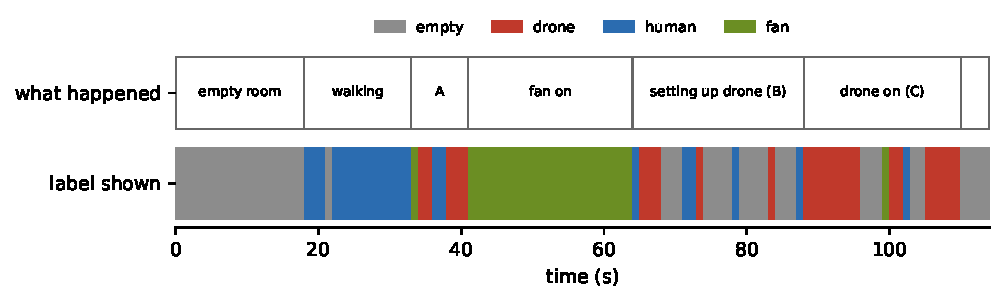
\includegraphics[width=\linewidth]{figs/live_timeline.pdf}
\caption{Labels shown in the first live session (top row read from a screen recording, one per second) against what happened (bottom row). A: switching the fan on close to the radar. B: setting up the drone. C: drone running; the two short ``empty'' gaps are moments when a propeller stalled.}
\label{fig:live}
\end{figure}

\paragraph{Replay of every recording through the final live classifier.} To measure the effect of the smoothing rules, every recording was replayed frame by frame through the live classifier, using a model trained on all \emph{other} recordings (Figure~\ref{fig:replay}, Table~\ref{tab:replay}). The smoothing thresholds themselves were chosen on these recordings, so this too is not an independent test.

\begin{table}[h]\centering\small
\caption{Leave-one-recording-out replay, share of frames per output label (\%), per window (raw) and with the final smoothing.}\label{tab:replay}
\begin{tabular}{@{}llrrrrr@{}}\toprule
True class & Version & drone & human & fan & empty & unsure\\\midrule
empty & raw / smoothed & 0 / 0 & 0 / 0 & 0 / 0 & 100 / 100 & -- / 0\\
human & raw / smoothed & 5.1 / 0 & 89.9 / 84.6 & 1.0 / 0 & 4.1 / 4.1 & -- / 11.4\\
fan & raw / smoothed & 3.4 / 0 & 0 / 0 & 96.6 / 90.3 & 0 / 0 & -- / 9.7\\
drone (all six) & raw / smoothed & 65.9 / 58.7 & 11.3 / 9.3 & 0.5 / 0 & 22.3 / 22.3 & -- / 9.7\\\bottomrule
\end{tabular}\end{table}
\begin{itemize}
\item Without smoothing, people were labelled ``drone'' in 5.1\,\% of frames and fans in 3.4\,\%. With the final rules, \textbf{no frame of the person, fan or empty-room recordings in this data set was labelled ``drone''}. This is a statement about these 22 recordings, not a guaranteed false-alarm rate.
\item The price is the ``unsure'' label: 11\,\% of human and 10\,\% of fan frames. Most of it comes from the harder recordings listed above; a small part comes from the start of every recording, where the smoother waits for three predictions before it gives a label (the first three frames, before the first one-second window is complete, are not scored at all). Correct labels are lost too: the drone label drops from 65.9 to 58.7\,\% of drone frames.
\item The decision also comes later. From a cold start, the first ``drone'' label appeared after 4 frames (1.0\,s) without smoothing and after 6 frames (1.5\,s) with it, in all four tethered-drone recordings. After a change of scene the two-second average can delay a change of label by up to about two seconds; I did not measure this directly.
\item Tethered-drone recordings within \SI{1.2}{m} were labelled ``drone'' in 94 to 98\,\% of frames, and 75\,\% for the moving one. The drone total in Figure~\ref{fig:replay} is lower because it includes the free flight and the out-of-range recording at \SI{1.9}{m}.
\item Empty-room recordings: 100\,\% ``empty'' in both versions.
\end{itemize}

\begin{figure}[t]
\centering
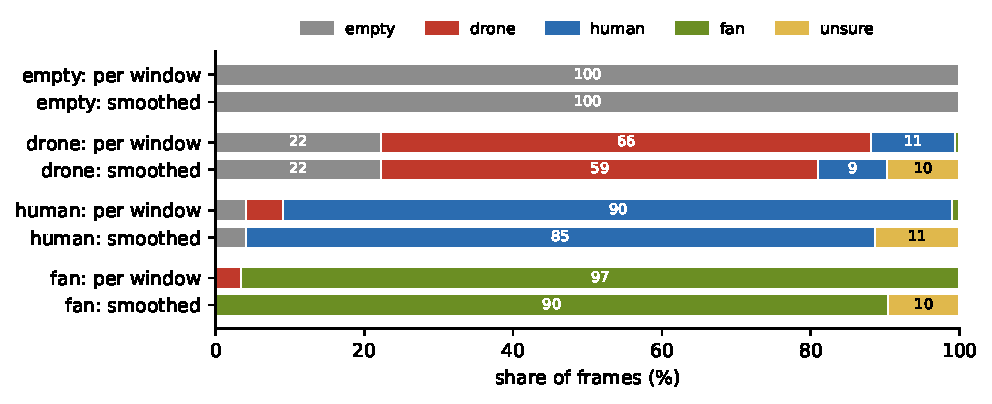
\includegraphics[width=0.92\linewidth]{figs/replay.pdf}
\caption{Leave-one-recording-out replay of all 28 recordings through the live classifier, frame by frame. ``Per window'': raw prediction. ``Smoothed'': two-second probability average, 60\,\% confidence (70\,\% for drone) or ``unsure''.}
\label{fig:replay}
\end{figure}

\subsection{Simulation against measurement}\label{sec:sim}

The simulator is approximate: it treats every scatterer as stationary during a chirp, which for the simulated blade tips at about \SI{72}{m/s} ignores a phase change of about \SI{2.4}{rad} within the chirp, which shifts the beat frequency by nearly 0.4 of a range bin, and it combines the antennas differently from the board. Figure~\ref{fig:sim} compares the measured spectrum of the drone tethered at a nominal \SI{0.5}{m} (radar range \SI{0.59}{m}) with the simulator, using the same chirp and a drone model with four two-blade rotors of \SI{2.3}{cm} radius at 500 revolutions per second. The simulation reproduces the main fact: energy over the full velocity axis, because the tips alias. It does not reproduce the detail. The simulated spectrum is much more structured, with sharp lines and deep notches, while the measured one is smoother. Real blades are not lines of point scatterers, the four motors do not turn at exactly constant speed, and the drone vibrates; all three smear the lines out. The rotation rate of the real motors is also unknown (Section~\ref{sec:next}). In short, the simulator was right about what kind of signature to look for and wrong about its fine structure, which is consistent with the weak performance of the line-based features.

\begin{figure}[t]
\centering
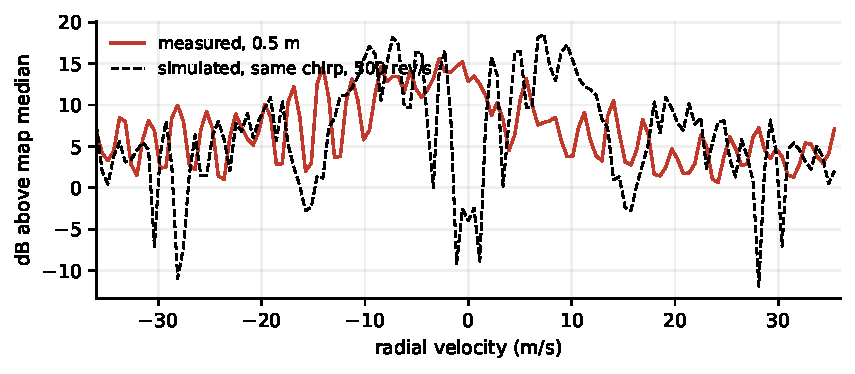
\includegraphics[width=0.9\linewidth]{figs/sim_vs_meas.pdf}
\caption{Doppler spectrum of the tethered drone, measured and simulated with the same chirp. The simulated curve is shifted to the same median level.}
\label{fig:sim}
\end{figure}

\subsection{What went wrong, and what it taught me}\label{sec:wrong}

\begin{itemize}
\item \textbf{Fixed artefacts near the radar.} Every recording, including the empty room, shows fixed spots very close to the radar: at zero velocity in the first range bin, and at about $-21$ to $\SI{-24}{m/s}$ between 0.1 and \SI{0.35}{m} (visible in Figure~\ref{fig:rd}). Their source is unknown to me; they are probably internal coupling in the board. Because they fall in the skirt band, they made targets close to the radar look drone-like until everything closer than \SI{0.45}{m} was excluded from the target search.
\item \textbf{The fast fan.} Before two side-on recordings of the fan (settings 1 and 3) were added, the model was unsure about the setting-3 fan at \SI{1}{m} in 79\,\% of frames; afterwards in 3\,\%. A fast fan really does put energy closer to the skirt band, and the model needed to see it.
\item \textbf{Slow movement.} Velocities within two Doppler bins of zero ($|v| \le \SI{1.1}{m/s}$) were first ignored altogether, which hid a person standing almost still. Ignoring only $|k| \le 1$ (below \SI{0.56}{m/s}) and lowering the gate from 9 to \SI{8}{dB} raised the share of human frames recognised from 70\,\% to 85\,\%, with the empty room still at 100\,\%. It also let a few false drone labels back in, which is why ``drone'' now needs 70\,\% confidence.
\item \textbf{A recording that was wrongly labelled.} One ``drone'' recording turned out to have been taken while the drone failed to start (1.8\,\% of its windows above the gate). It was removed from the data set; with the gate it is easy to spot such recordings.
\end{itemize}

%=====================================================================
\section{Radar analysis: scale, link budget and detection}\label{sec:analysis}
%=====================================================================

This section looks at the measurements as a radar engineer would: what the numbers on the map mean physically, whether the echo strength agrees with the radar equation, how large the drone looks to the radar, and what actually limits the range.

\subsection{What one decibel on the map means}\label{sec:scale}

The firmware does not document the scale of the range-Doppler map precisely, so I checked it with two independent tests.

\paragraph{Noise statistics.} After the two FFTs, thermal noise in one antenna is complex Gaussian. The logarithm of its magnitude, $20\log_{10}|X|$, then has a known distribution: a standard deviation of \SI{5.57}{dB} and a long tail towards low values. If the firmware averages the log-magnitudes of the four antennas, the standard deviation falls to \SI{2.78}{dB} and the skewness to $-0.56$. In the five empty-room recordings, map cells away from zero velocity and from the board's artefacts have a standard deviation of 1.46 map units and a skewness of $-0.52$. The \emph{shape} matches four averaged antennas; the \emph{scale} is smaller by a factor of 1.91 (Figure~\ref{fig:scale}, left).

\paragraph{The radar equation.} For a point-like target the echo power falls as $R^{-4}$. I measured the total drone echo at its range row (the row the drone occupies most often in the recording; the moving Doppler bins summed in linear units, minus the same sum averaged over rows far from the drone) at three ranges. Taking map units as dB, it falls by only \SI{15.3}{dB} from \SI{0.59}{m} to \SI{1.87}{m}, much less than the \SI{20.0}{dB} of the $R^{-4}$ law, which is implausible for a target much smaller than the beam. Recomputing the same sum with every cell rescaled by a factor $K$ (true dB per map unit) gives a fall of 18.5, 20.3, 21.4 and \SI{22.2}{dB} for $K = 1.5$, 1.75, 1.9 and 2 (Figure~\ref{fig:scale}, right). The radar equation is matched best by $K \approx 1.75$. The weakest of the three points lies only 3 to \SI{9}{dB} above what the same estimator returns in the empty room (Section~\ref{sec:rcs}), so it may be overestimated; a lower value there would favour a smaller $K$. Because $K$ was chosen on these three recordings, they cannot also validate it. Two pairs from the independent test give a separate check: the drone on the same pole at 0.82 and \SI{1.41}{m} (T09, T10) falls by \SI{9.3}{dB} for $K = 1.65$ against \SI{9.4}{dB} predicted, while the drone on a sofa arm at 1.29 and \SI{1.64}{m} (U05, U04) falls by 8 to \SI{10}{dB} against \SI{4.2}{dB} predicted for any $K$ in the range, so placement and viewing angle change the echo by several decibels.

Taken together, one map unit corresponds to roughly 1.65 to 1.9 true dB, which I round to ``about two'' in this report. This is an empirical factor. The most likely explanation is a fixed-point format or antenna combination different from the one assumed in the conversion, but I have not confirmed it in the firmware source. An earlier version of this check clipped the per-bin excess over the noise at zero; that keeps positive noise fluctuations, biased the weakest point upwards by 1.6 to \SI{3.4}{dB} and made the agreement look tighter than it is.

\begin{figure}[t]
\centering
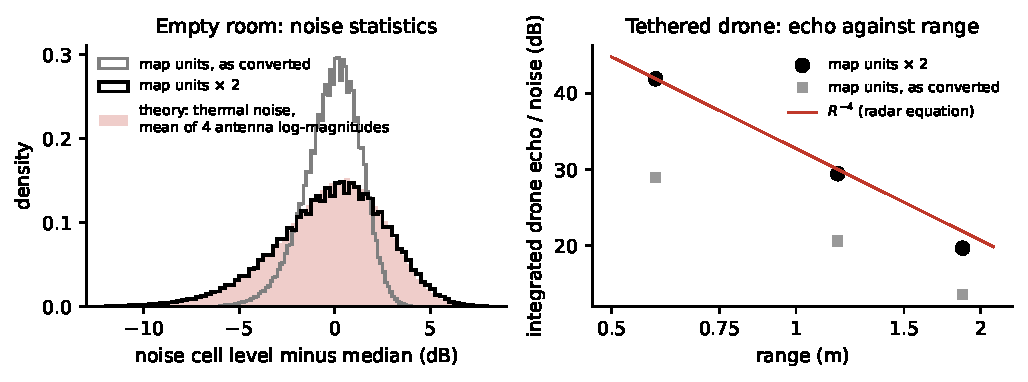
\includegraphics[width=0.98\linewidth]{figs/scale.pdf}
\caption{Left: noise cells of the empty-room maps compared with the theoretical distribution for thermal noise averaged over four antennas. Right: total drone echo at three ranges, noise subtracted. On the map scale the echo falls far too slowly; with the map rescaled by two it falls \SI{2.2}{dB} faster than the radar equation; the best match is a factor of about 1.75.}
\label{fig:scale}
\end{figure}

\subsection{Link budget and the radar cross section of the drone}\label{sec:rcs}

The datasheet of the IWR6843AOP \cite{ti-ds} gives the transmitter output as an effective isotropic radiated power (EIRP) of \SI{16}{dBm} and the receiver as an effective isotropic noise figure (EINF) of \SI{9}{dB}, both typical values that already include the antenna gains. Written in these terms, the radar equation for the signal-to-noise ratio after both FFTs is
\begin{equation}
\mathrm{SNR} = \frac{\mathrm{EIRP}\;\sigma\;\lambda^2\;T_{\mathrm{obs}}}{(4\pi)^3\,R^4\;k T_0\;\mathrm{EINF}},
\end{equation}
where $T_{\mathrm{obs}} = N\,T_{\mathrm{adc}} = 128 \times \SI{12.8}{\micro s} = \SI{1.64}{ms}$ is the time over which the signal is coherently integrated, $k T_0 = \SI{4.0e-21}{W/Hz}$ is the thermal noise density, and $\sigma$ is the radar cross section (RCS). The integration time appears because the two FFTs add up all samples coherently: the signal grows with their number, the noise only with its square root. For $\sigma = \SI{1}{m^2}$ at \SI{1}{m} this gives \SI{74}{dB}, or about \SI{70}{dB} after a window loss of \SI{3.5}{dB}, the value for two Hann windows. The firmware in fact uses a Blackman window in range and a Hann window in Doppler, which together lose about \SI{4.1}{dB}; the cross sections below are therefore about \SI{0.6}{dB} (15\,\%) too low.

Comparing this with the measured total echo of the tethered drone gives an estimate of its RCS. It depends on the scale factor $K$:
\begin{center}\small
\begin{tabular}{@{}lccc@{}}\toprule
Range & \SI{0.59}{m} & \SI{1.17}{m} & \SI{1.87}{m}\\\midrule
Total echo over noise, $K=2$ (dB) & 41.9 & 29.4 & 19.7\\
Implied RCS, $K=2$ & \SI{-37.8}{dBsm} & \SI{-38.3}{dBsm} & \SI{-39.9}{dBsm}\\
Implied RCS, $K=1.75$ & \SI{-41.2}{dBsm} & \SI{-40.5}{dBsm} & \SI{-41.3}{dBsm}\\\bottomrule
\end{tabular}
\end{center}
The four tethered recordings of the independent test give $-37.7$ to \SI{-44.3}{dBsm} for $K$ between 1.65 and 1.9. Over all seven recordings and that range of $K$, the estimate lies between about $-38$ and \SI{-44}{dBsm}, i.e.\ 0.4 to \SI{1.7}{cm^2}: of the order of \SI{1}{cm^2}, with a spread of more than a factor of four before the datasheet uncertainties are counted. Because the tethered drone's body is static and removed by the clutter filter, this is an effective cross section of the moving return, mostly the four spinning propellers; body vibration and multipath may also contribute. The estimator sums the moving Doppler bins of the target's range row only. The echo also leaks into the two neighbouring rows (through the range window and the target's own extent); including them raises it by 2.5 to \SI{3.3}{dB} in all seven recordings. The link budget's \SI{3.5}{dB} window loss assumes peak-cell values in both dimensions, whereas the Doppler bins are summed, and the map combines the antennas in the log domain, so this accounting is approximate to a few decibels. Because the neighbour-row offset is nearly the same in every recording, it does not affect the $R^{-4}$ check or the choice of $K$. This is a model-dependent estimate, not a calibrated measurement, and it is uncertain by several decibels: the datasheet values are typical rather than measured for this board, the window loss is estimated, the scale factor is empirical, the map median is not exactly the mean noise power, and averaging log-magnitudes over antennas does not give the arithmetic antenna power. The agreement between the three training distances (within 0.8 to \SI{2}{dB}, depending on $K$) is not independent evidence, because the same three recordings were used to choose $K$; the test recordings show that a different placement alone can move the estimate by 4 to \SI{5}{dB}. The estimator is also affected by a selection bias. Applied to the nine empty-room recordings, where there is no target, it returns an apparent echo of 9 to \SI{18}{dB} ($K$ = 1.65 to 2), because the row it fixes is then itself a noise peak or the weak echo at about \SI{6}{m} (Section~\ref{sec:test}). For the drone the row is set by the target (the same row in 68 to 100\,\% of frames), so the bias should be smaller, but the two weakest points (\SI{1.87}{m} and \SI{1.64}{m}) lie only 3 to \SI{10}{dB} above the empty-room values of their rooms and may be overestimated by a few decibels. The empty-room values are not a correction that could simply be subtracted. The 0.4 to \SI{1.7}{cm^2} above is therefore a spread of model-dependent estimates, not a confidence interval. A reference reflector of known RCS would be needed for a calibrated value. For comparison, the moving parts of a walking person give $-10$ to \SI{-15}{dBsm} (row and range taken frame by frame; the spread depends on how a strongly fluctuating echo is averaged), some 25 to 30\,dB more than the propellers.

The same numbers predict the range of the detection gate. The gate requires a one-second mean of the peak SNR of 8 map units, i.e.\ \SI{16}{dB} true. The tethered drone had \SI{22.4}{dB} at \SI{1.17}{m}; with $R^{-4}$ this falls to \SI{16}{dB} at about \SI{1.7}{m} (about \SI{1.6}{m} if $K$ is 1.65 to 1.75), which is where the gate should stop detecting it.

\subsection{Detection: what limits the range}\label{sec:det}

\paragraph{The gate as a detector.} Figure~\ref{fig:det} (left) shows, for every threshold, the share of empty-room windows above it (false alarms) and the share of drone windows above it (detections). At the chosen \SI{16}{dB} no empty window was above the threshold. With 517 empty-room frames, i.e.\ about 129 non-overlapping windows, this would bound the false-alarm rate per window at about 2\,\% with 95\,\% confidence (zero events in $n$ trials bound the rate by $3/n$) if the windows were independent and the threshold had been fixed in advance. Neither is true here: neighbouring windows are correlated, and the gate was chosen on these same recordings. The number is illustrative only; the independent test (Section~\ref{sec:test}) is the better check. The drone at 0.6 and \SI{1.2}{m} is above the threshold in every window, at \SI{1.9}{m} in none.

\paragraph{Why the gate fails at 1.9 m.} The gate looks at the peak of the range row with the most moving energy (and its two neighbours), chosen \emph{anywhere} beyond \SI{0.45}{m}. In an empty room this is close to the maximum of several thousand noise cells, which is much higher than a typical noise cell, and in the first empty recordings it was also a weak moving object at about \SI{6}{m}, outside the area of interest. Looking only at the three range cells around the drone at \SI{1.9}{m} tells a different story (Figure~\ref{fig:det}, right). In single frames, the empty room reaches at most \SI{9.3}{dB} in those cells, while the drone's median is \SI{13.4}{dB}; 97\,\% of the drone frames are above the highest empty-room value.

\paragraph{Averaging frames.} Averaging the power of $N$ consecutive maps does not change the mean level of the drone but reduces the random fluctuation of the noise by about $\sqrt{N}$. This is non-coherent integration. The highest empty-room value at the drone cells falls from 9.3 to \SI{3.6}{dB} after two seconds, while the drone stays near \SI{12}{dB}; the margin between them grows from 4 to \SI{8}{dB}, and to \SI{10}{dB} after eight seconds. From 1 to 32 frames the margin grows by \SI{5.8}{dB}. This is an observed margin, not an integration gain at a fixed false-alarm probability: the longer the average, the fewer empty-room values there are to take the maximum of (517 single frames, but only 13 averages of 32), and a smaller sample by itself tends to have a lower maximum.

\paragraph{What this means.} With this chirp, the range is limited at least as much by the simple detector as by the physics. A detector that compares every range cell with its own noise level (a constant-false-alarm-rate, or CFAR, detector) and averages about one second might detect the tethered drone at \SI{1.9}{m}, where the global gate failed; whether it would reach further has not been measured. Two caveats: here the cells were chosen knowing where the drone was, whereas a real detector tests every cell and its false-alarm rate grows with the number of cells; and the result rests on one recording. It is a prediction to test, not a measured range.

\begin{figure}[t]
\centering
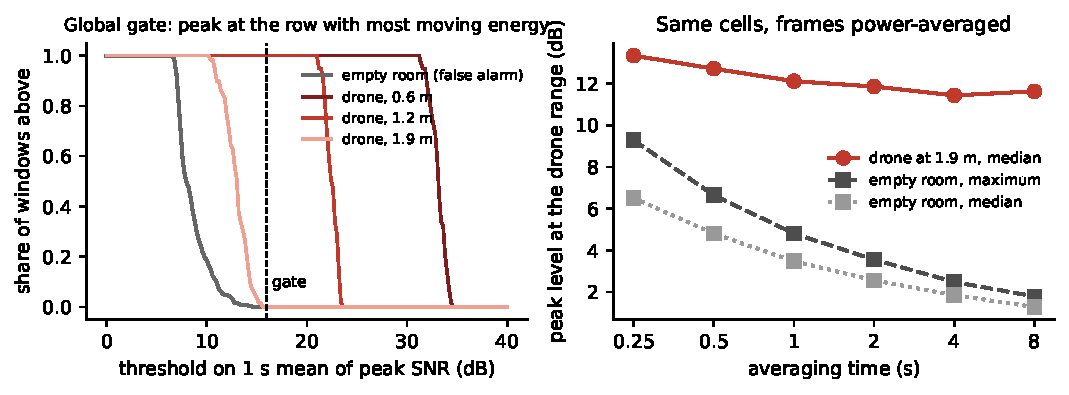
\includegraphics[width=0.98\linewidth]{figs/detection.pdf}
\caption{Left: share of one-second windows above a threshold, for the empty room and for the tethered drone at three ranges (thresholds in true dB), using the implemented gate: the peak SNR in the row with the most moving energy and its two neighbours. Right: the drone at \SI{1.9}{m} against the empty room, in the same three range cells, after power-averaging frames.}
\label{fig:det}
\end{figure}

%=====================================================================
\section{Independent test with a frozen model}\label{sec:test}
%=====================================================================

Every number so far comes from recordings that were also used to choose the features, the gate and the thresholds (Section~\ref{sec:classif}). To get one result that was not tuned, I froze the system and recorded new data.

\paragraph{Protocol.} The final model was trained once on all 28 labelled recordings; the random forest itself sees the 988 windows above the gate, which come from 22 of them (the five empty rooms and the drone at \SI{1.9}{m} have none). The model file, the classification code (\texttt{classify.py}, \texttt{features.py}, \texttt{config.py}) and the chirp configuration were then fixed and their checksums written to a manifest. In a separate session I made new recordings in the training room (room~1) and in a second room that the system had never seen (room~2, a living room of about \SI{18}{m^2} with sofas and a carpet). Each recording was evaluated once by a script that first compares the frozen files with the manifest and stops if anything differs, and then plays the recording frame by frame through the live classifier with its gate and smoothing. Nothing was changed after looking at a test result. Some files outside the frozen set did change after freezing, none of them in a way that affects how stored recordings are read or classified: \texttt{record.py} and \texttt{session.py} (new recordings are numbered instead of time-stamped; malformed files are rejected when loading), \texttt{tlv.py} (stricter checks on malformed packets, used only when reading from the board), input checks in \texttt{phase.py} and \texttt{check\_board.py}, and console messages and comments in a few others. For publication, comments were later removed from the frozen files. The published manifest therefore lists the checksums of the published files, and the checksum check in the repository (\texttt{mmwd/freeze.py}) only shows that the current files match that manifest; it is not proof of what ran on the test day. The original checksums, against which the test-day check passed, are kept in a second file, but the original files are not published, so a reader cannot repeat that check; the repository has no commit made before the test. The model file itself is unchanged (its checksum is the same in both lists), and the published code and model reproduce every test result exactly. That the test used these files before any result was seen rests on my account, not on evidence a reader can verify.

The test set has 20 recordings (T01 to T13 in room~1, U01 to U07 in room~2). One further fan recording, made while the radar was \SI{18}{cm} lower than in training (T03x), is reported as its own condition. Four more were set aside before scoring: one made with the radar facing the wrong way, one with no frames because the USB connection dropped, one in which no propeller echo was present at the drone's range (whether the drone had stopped, was at low throttle or was outside the beam is not known, so its outputs, 98\,\% person, cannot be scored as right or wrong; they are kept and discussed below), and a ten-second check of the table set-up before the repeat. All are kept in the repository; none of them contains a drone label for a non-drone scene. One walking recording that was cut at \SI{18}{s} by a connection drop is kept in the test set.

\begin{figure}[t]
\centering
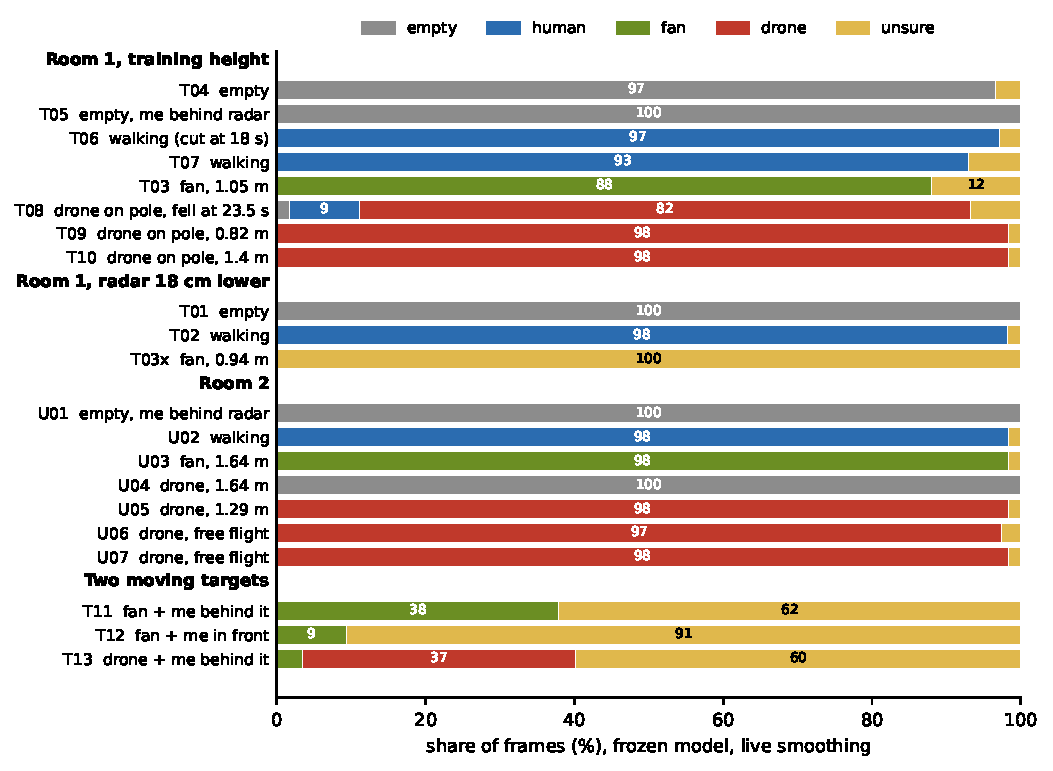
\includegraphics[width=0.94\linewidth]{figs/test.pdf}
\caption{Independent test: output of the frozen live classifier on every new recording, as a share of frames. Ranges are those measured by the radar.}
\label{fig:test}
\end{figure}

\paragraph{One target at a time.} Figure~\ref{fig:test} and Table~\ref{tab:test} show the result. In the ten recordings without a drone (four empty rooms, four walking, two fans; 1110 frames, both rooms and both radar heights) not a single frame was labelled as a drone. Empty rooms were labelled empty in 99\,\% of frames, walking in 97\,\% and fans at the training height in 93\,\% (T03 and U03); the rest was ``unsure''. With the radar \SI{18}{cm} lower (T03x, below), the same fan was never labelled as a fan: 0\,\% fan, 100\,\% ``unsure''. Pooled with that recording, fans were labelled as fans in 62\,\% of frames, a number that hides this complete failure under the changed geometry. Seven single-target drone recordings were made; six of them at measured ranges of 0.82 to \SI{1.41}{m}. In five of these (T09, T10, U05, U06, U07), 98\,\% of 583 frames were labelled as a drone, in both rooms; the sixth (T08) is the recording in which the drone fell (below). Over all six, 668 of 700 frames (95\,\%) were labelled as a drone; counting only the frames in which the drone was on its mount or in flight (T08 up to its fall), 661 of 674 (98\,\%). Three of these were held in place (on the pole in room~1, on the arm of a sofa in room~2) and two were free flights in room~2, in which the drone moved between about 0.6 and \SI{1.3}{m}. In the training data the one free flight was recognised in only 10\,\% of windows; that flight drifted further and less steadily, so two short flights close to the radar do not show that free flight is solved, only that it works in this range. In one tethered recording the drone fell off the pole near the end; the moment is visible in the data at \SI{23.5}{s}, when the measured range leaves the bin it held from the start. Before that, 98\,\% of frames were labelled as a drone; over the whole recording, 82\,\%.

\paragraph{The range limit, in a new room.} Section~\ref{sec:rcs} predicted that the global gate would lose the drone at about \SI{1.6}{} to \SI{1.7}{m}. In room~2 the drone at a measured \SI{1.64}{m} was labelled ``empty'' in every frame: its strongest one-second window reached \SI{7.5}{dB}, just under the \SI{8}{dB} gate. In its own range cell the drone was still visible, about \SI{3}{dB} above the neighbouring cells, which again points at the gate, not the radar, as the limit.

\paragraph{The empty-room margin.} In room~2 the strongest empty-room window was \SI{4.3}{dB}, well under the gate. In room~1 one empty recording reached \SI{8.1}{dB}, \SI{0.1}{dB} over the gate, and 3\,\% of its frames became ``unsure''. The cause was a weak moving echo at about \SI{6}{m} with a slowly decreasing velocity, which also appeared in the recording made with the radar facing the wrong way and in some training recordings. Its source is not known. The room is shorter than \SI{6}{m}, so it is either a reflection or something outside the room; in both recordings in which it was strong I had left the room and was outside the closed door, and in the next empty recording, with me standing behind the radar inside the room, it was gone. The gate margin in this room is therefore small.

\paragraph{Radar height.} The first three recordings of the test set were made, by mistake, with the radar \SI{18}{cm} lower than during training. The empty room and the walking person were unaffected (100 and 98\,\%). The fan at \SI{1}{m} was not: 0\,\% of frames were labelled as a fan and 100\,\% ``unsure''. Its echo was about \SI{4.5}{dB} stronger than in any training fan recording and had a smaller share of high velocities, so the model, which had never seen a fan from this angle, gave fan and drone equal probability. After the radar was raised to the training height, the same fan was labelled as a fan in 88\,\% of frames. The classifier is sensitive to the viewing geometry of a fan; in this case it abstained instead of raising a false alarm.

\paragraph{Drone on a table.} The three intact-propeller recordings of Section~\ref{sec:prop}, made with the drone taped to a table and never used for training, give a further check: 29 to 78\,\% of their frames were labelled as a drone and the rest ``unsure''; none was labelled as another class. The table and the different mounting change the signature enough to cost confidence.

\paragraph{Two moving targets.} The classifier describes one range row only: the one with the most moving energy, together with its two neighbours (Section~\ref{sec:features}). Three recordings test what happens when there are two moving objects. With the fan at \SI{1.17}{m} and me walking on the spot 1.5 to \SI{2}{m} behind it and to one side, the fan's row was selected in every frame; 38\,\% of frames were labelled fan and 62\,\% ``unsure'', presumably because my motion leaked into the fan's spectrum. With me in front of the fan at \SI{0.7}{m}, the two echoes were about equally strong, the selected row jumped between us (fan in 72\,\% of frames), and 91\,\% of frames were ``unsure''. With the drone on a table at \SI{0.9}{m} and me walking on the spot about \SI{1.6}{m} away, the drone's row was selected in 56\,\% of frames, and 37\,\% of frames were labelled as a drone, 60\,\% ``unsure'' and 3\,\% fan. I had predicted from the average signal levels that I would mask the drone completely; that was wrong, because the echo of a person walking on the spot fluctuates from step to step while the drone's is steady. A first attempt at the drone-and-person scene (T13x, set aside) is not counted: no propeller echo was visible at the drone's range, and since it is not known whether the drone was running, its labels (98\,\% person, no drone) cannot be scored as right or wrong. In the two scenes with a fan and a person no frame was labelled as a drone. In the drone-and-person scene the 43 drone labels cannot all be attributed to the drone: in 16 of them the row selected in the current frame (the one with the most moving energy) lay at the person's range (1.41 to \SI{1.64}{m}). In none of these 16 did all four frames of the one-second window lie at the person's range, so the window, and then the smoothing, mixed frames from both targets; the labels belong to the scene, not to one object. Only the scene-level shares are meaningful here, and the design clearly reaches its limit: mixed scenes mostly end as ``unsure''. The obvious remedy is to classify every range row with moving energy separately instead of only one.

\begin{table}[t]
\centering\scriptsize
\caption{Independent test with the frozen model. Range: median range measured by the radar (10th to 90th percentile where it varied). Labels: share of frames output by the live classifier. Rec.\ T03x was made with the radar \SI{18}{cm} lower than in training (as were T01 and T02).}
\label{tab:test}
\begin{tabular}{@{}llllrrrrr@{}}
\toprule
Rec. & Room & Scene & Range (m) & empty & unsure & human & fan & drone\\
\midrule
T01 & 1, low & empty & -- & 100 & 0 & 0 & 0 & 0\\
T02 & 1, low & walking & 2.23 (1.64--2.93) & 0 & 2 & 98 & 0 & 0\\
T03x & 1, low & fan, setting 3 & 0.94 (0.94--1.05) & 0 & 100 & 0 & 0 & 0\\
T03 & 1 & fan, setting 3 & 1.05 & 0 & 12 & 0 & 88 & 0\\
T04 & 1 & empty & -- & 97 & 3 & 0 & 0 & 0\\
T05 & 1 & empty, me behind radar & -- & 100 & 0 & 0 & 0 & 0\\
T06 & 1 & walking (18\,s) & 2.34 (1.87--3.03) & 0 & 3 & 97 & 0 & 0\\
T07 & 1 & walking & 2.46 (1.99--3.04) & 0 & 7 & 93 & 0 & 0\\
T08 & 1 & drone on pole, fell at 23.5\,s & 0.82 & 2 & 7 & 9 & 0 & 82\\
T09 & 1 & drone on pole & 0.82 & 0 & 2 & 0 & 0 & 98\\
T10 & 1 & drone on pole & 1.41 (1.29--1.41) & 0 & 2 & 0 & 0 & 98\\
T11 & 1 & fan + me 1.5--2\,m behind & 1.17 & 0 & 62 & 0 & 38 & 0\\
T12 & 1 & fan + me 0.7\,m in front & 1.17 (0.70--1.17) & 0 & 91 & 0 & 9 & 0\\
T13 & 1 & drone on table + me behind & 0.94 (0.94--1.64) & 0 & 60 & 0 & 3 & 37\\
U01 & 2 & empty, me behind radar & -- & 100 & 0 & 0 & 0 & 0\\
U02 & 2 & walking & 2.23 (1.64--2.69) & 0 & 2 & 98 & 0 & 0\\
U03 & 2 & fan, setting 3 & 1.64 & 0 & 2 & 0 & 98 & 0\\
U04 & 2 & drone on sofa arm & 1.64 (1.64--2.87) & 100 & 0 & 0 & 0 & 0\\
U05 & 2 & drone on sofa arm & 1.29 & 0 & 2 & 0 & 0 & 98\\
U06 & 2 & drone, free flight & 0.94 (0.82--1.05) & 0 & 3 & 0 & 0 & 97\\
U07 & 2 & drone, free flight & 1.05 (0.82--1.17) & 0 & 2 & 0 & 0 & 98\\
\bottomrule
\end{tabular}
\end{table}

\paragraph{What the test does and does not show.} It shows that the frozen system, without any change, kept its behaviour on new recordings and in a new room: no false drone in 1110 frames of empty rooms, people and fans, 98\,\% of frames correct in five near-range drone recordings, and 82\,\% in a sixth in which the drone fell off its pole. It does not show that it works for another drone, another person or another fan, which were the same as in training. The frame shares come from overlapping windows of 21 recordings (the 20 test recordings and T03x) and should be read per recording, not as thousands of independent trials. In particular, no false drone in 1110 frames does not establish a zero false-alarm rate: consecutive frames are strongly correlated and each label uses a window of four frames smoothed over eight, so the evidence amounts to ten recordings of three kinds of scene, made by one person with one fan in two rooms. Even read as ten independent trials, zero failures only bound the per-recording failure rate at about 30\,\% with 95\,\% confidence. And the test exposed three weaknesses that the training data had hidden: sensitivity to the viewing angle of a fan, a small empty-room margin in room~1, and a single-target design that cannot separate two moving objects.

%=====================================================================
\section{Follow-up A: seeing a person who does not move}\label{sec:still}
%=====================================================================

A person sitting still is removed by static clutter removal, like the furniture. To see whether the radar can tell an occupied room from an empty one in that case, I switched clutter removal off (configuration \texttt{md\_breath.cfg}, otherwise identical) and looked at the \emph{range profile}, which the board sends every frame: the echo power in each range bin at zero velocity.

\paragraph{A still person is visible.} With clutter removal on (recording B01), the mean level of the range profile at my position was at the noise level, but it still fluctuated more than the same bin in the five empty-room recordings (standard deviation 2.3 against 1.1 to 1.5 map units). With clutter removal off (Figure~\ref{fig:still}), range bins containing only walls and furniture varied by about \SI{0.2}{dB} over a minute, while the bins where I stood still varied by 2 to \SI{5}{dB}. Breathing, small sway and the heartbeat move the body by millimetres, and at a wavelength of \SI{4.9}{mm} that is enough to change the interference between my echo and the static echoes in the same bin. This suggests that an occupied room can be told from an empty one even when nobody moves. The comparison here is between bins of the same occupied recording; an empty-room recording with clutter removal off, which would make it direct, was not made.

\begin{figure}[t]
\centering
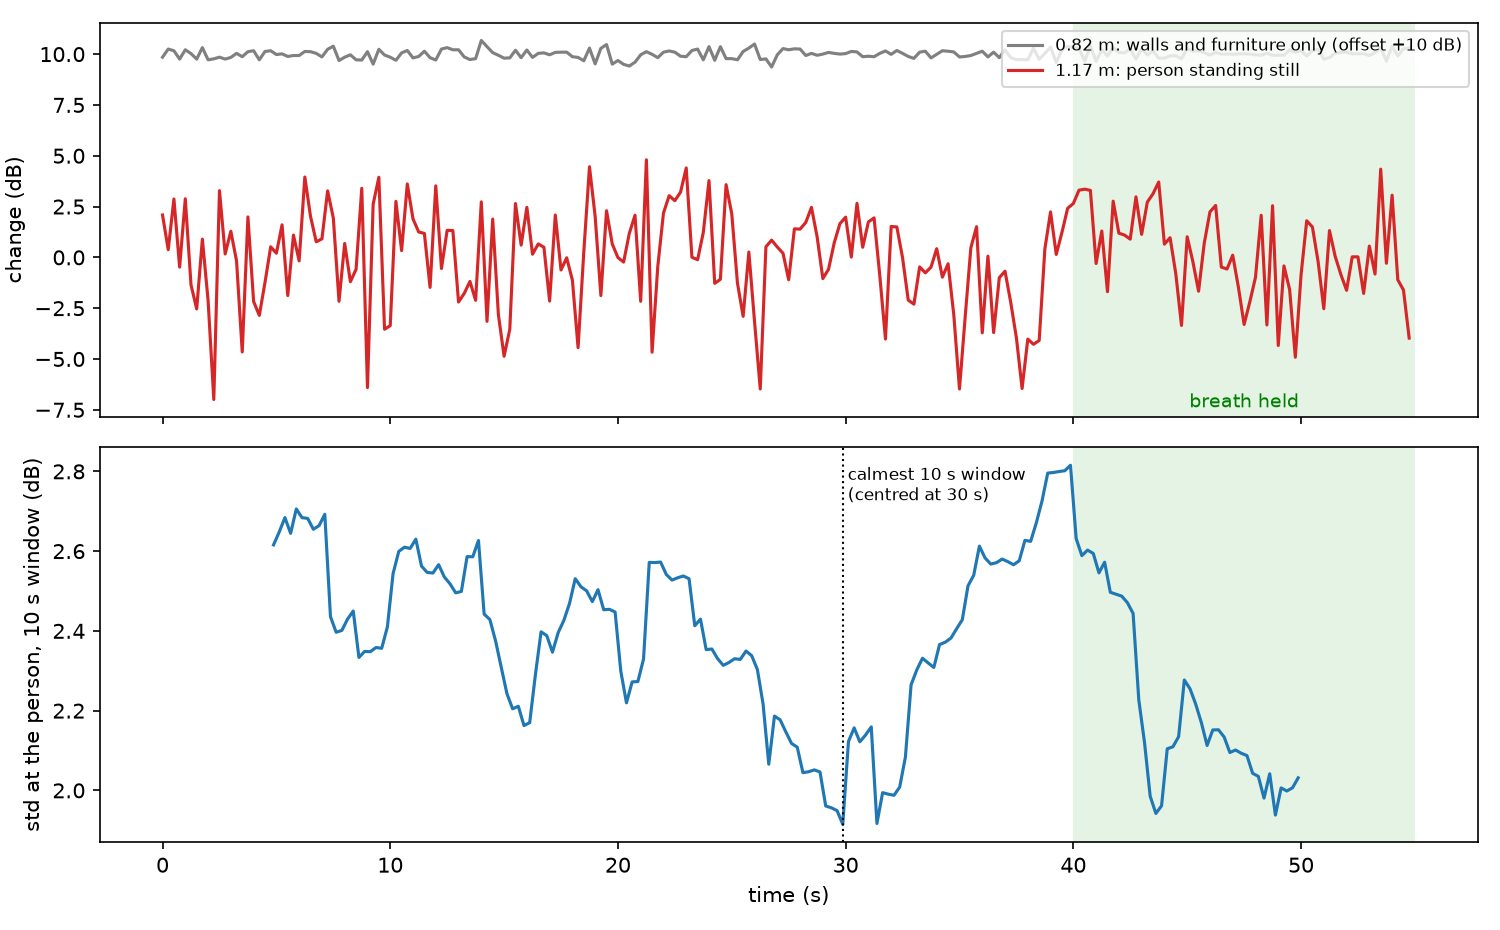
\includegraphics[width=0.85\linewidth]{figs/fig_breath_test.png}
\caption{Clutter removal off, four frames per second (recording B02: deep breathing from 0 to 40\,s, breath held from 40 to 55\,s, shaded). Top: a bin with only static objects (grey) against the bin where I stood still (red). Bottom: standard deviation at my range over a sliding 10\,s window. The calmest window is centred at 30\,s, during deep breathing, and the breath-hold period is not clearly calmer, so at this frame rate the recording does not show breathing.}
\label{fig:still}
\end{figure}

\paragraph{Faster frame rates.} At four frames per second a held breath was not clearly visible in the first recording (Figure~\ref{fig:still}). My first explanation was aliasing in slow time: a breath moves the chest by several millimetres, i.e.\ through several phase turns, so the echo power ripples a few times per second. A later check does not support this as the cause. Keeping every fifth sample of the 20-frame recording (i.e.\ four frames per second) still shows the held breath: the standard deviation of frame-to-frame changes at the chest is 3.1, 1.9 and 3.0 map units before, during and after the hold. The weak contrast of the four-frame recording therefore more likely comes from that take itself (deeper breathing, posture) than from the frame rate. For breathing the full range-Doppler map is not needed, so I made two more configurations that send only the range profile: 50\,ms frames (20 per second) and, with 32 chirps instead of 128, 20\,ms frames (50 per second). At 50 frames per second consecutive samples of the chest signal correlate at 0.94, against 0.50 at 20 frames per second (Figure~\ref{fig:sampling}), so the ripple is followed much more smoothly. This does not prove that it is free of aliasing, and the two were different recordings with different settings; part of the improvement may be due to calmer breathing in the 50-frame recording.

\begin{figure}[t]
\centering
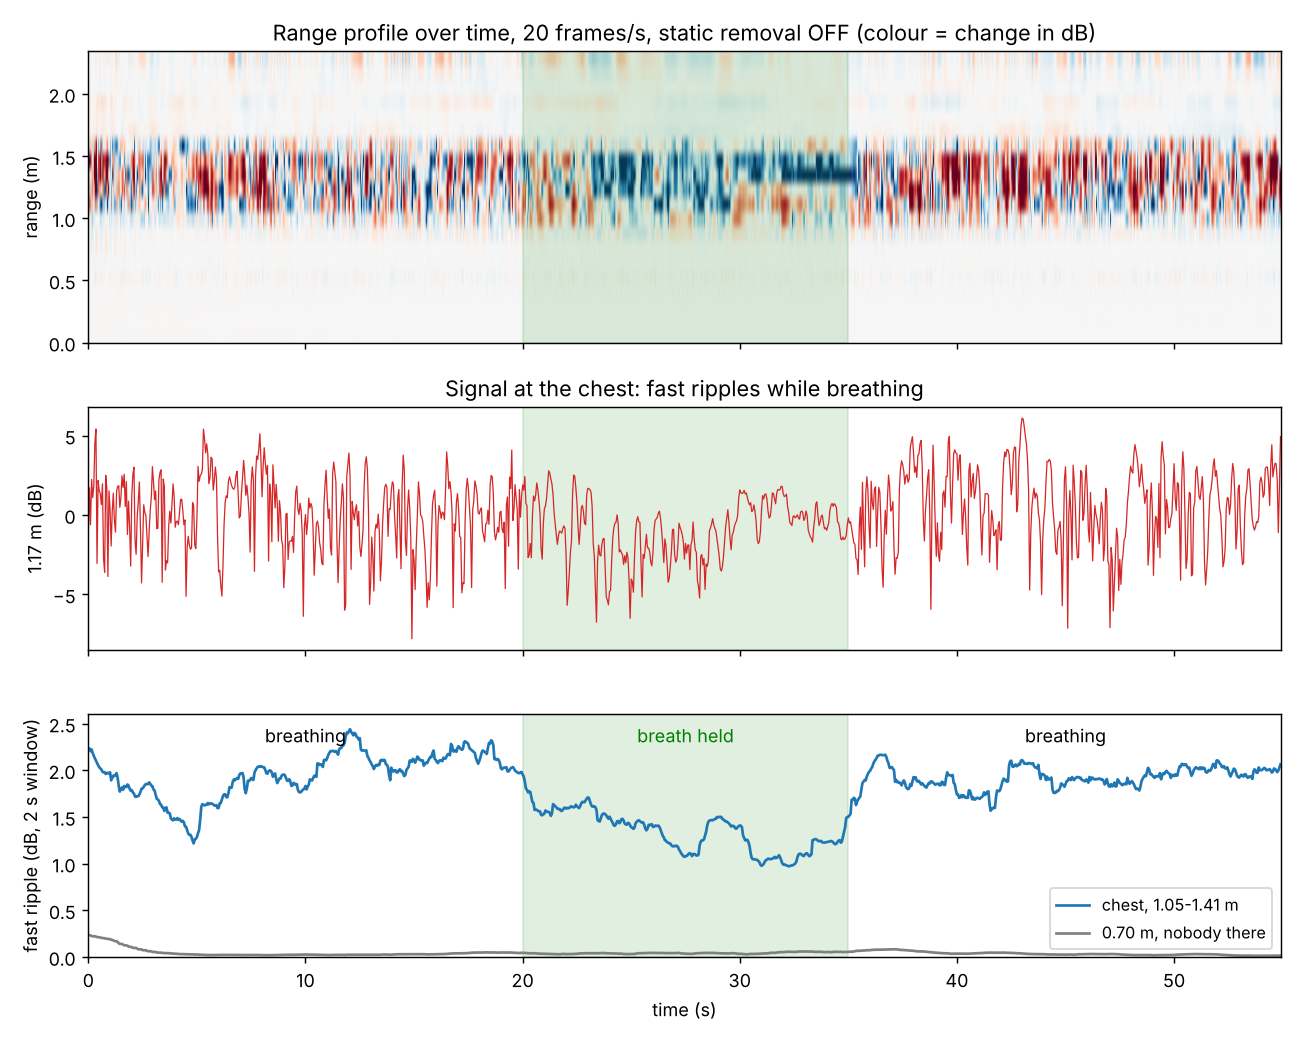
\includegraphics[width=0.85\linewidth]{figs/fig_breath_20fps.png}
\caption{Clutter removal off, 20 frames per second, standing about \SI{1}{m} from the radar, breath held from 20 to 35\,s. The fast ripple at the chest drops clearly while the breath is held and comes back as soon as breathing starts.}
\label{fig:breath}
\end{figure}

\begin{figure}[t]
\centering
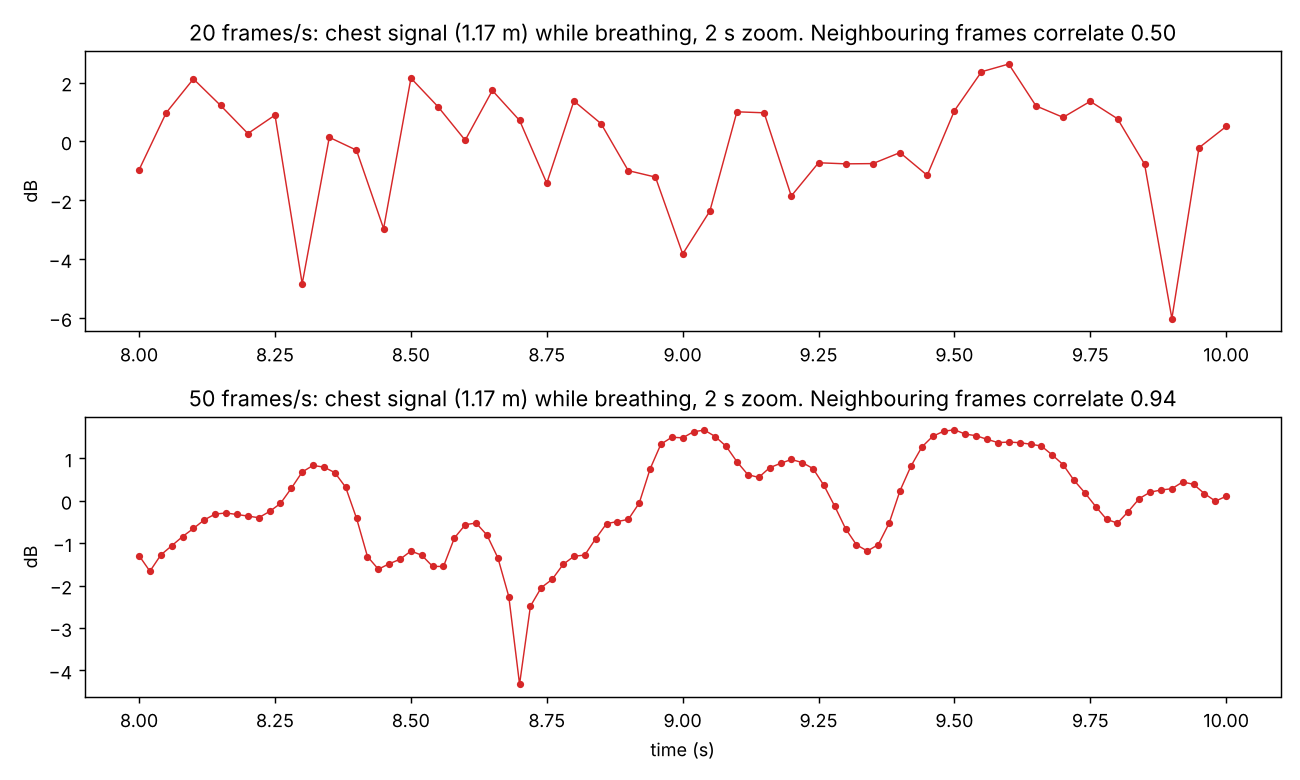
\includegraphics[width=0.82\linewidth]{figs/fig_breath_sampling.png}
\caption{Two seconds of the chest signal while breathing, at 20 and 50 frames per second.}
\label{fig:sampling}
\end{figure}

\paragraph{A held breath is visible.} In both faster recordings the fast ripple at the chest (power changes on time scales below one second) dropped while I held my breath and returned as soon as I breathed again (Figure~\ref{fig:breath}). At 20 frames per second the ripple fell on average by about a third, from \SI{2.0}{dB} to \SI{1.4}{dB}, and the power between 1 and \SI{5}{Hz} dropped to half. At 50 frames per second it fell from 1.7 to \SI{2.2}{dB} to 0.85 to \SI{1.2}{dB} in the three range bins covering my chest, roughly half. It does not drop to zero: the heart and small postural movements continue. These are two recordings of one person, so the result is ``breathing versus holding the breath can be distinguished'', not ``the breathing rate can be measured''.

%=====================================================================
\section{Follow-up B: getting the phase back}\label{sec:pr}
%=====================================================================

\subsection{Why this is a phase retrieval problem}

The breathing motion itself is in the \emph{phase} of the echo (Equation~\ref{eq:phase}): a chest displacement $d(t)$ rotates the phase by $\varphi(t) = 4\pi d(t)/\lambda$. The board sends only power. My bachelor's thesis was about exactly this situation, recovering a complex signal from magnitude-only measurements, so I tried to apply it.

For range bin $b$, receive antenna $k$, the echo is the sum of a moving part and a static part from everything else in the same bin:
\begin{equation}
X_{kb}(t) = A_{kb}\,e^{j\varphi(t)} + C_{kb}.
\end{equation}
If the board added the powers of the four antennas, the measurement would be
\begin{equation}
y_b(t) = \sum_k |X_{kb}(t)|^2 = \alpha_b + \operatorname{Re}\!\left(\gamma_b\,e^{j\varphi(t)}\right),\qquad
\alpha_b = \sum_k |A_{kb}|^2 + |C_{kb}|^2,\quad \gamma_b = 2\sum_k A_{kb}\overline{C_{kb}},
\label{eq:prmodel}
\end{equation}
the same structure as $y = |\langle a, x\rangle|^2$ in the thesis: only intensities are measured, the phase of $X$ itself is lost, and $\varphi(t)$ survives only inside the interference term. The static clutter $C$ acts like the reference wave in holography. One bin alone gives only $\cos(\varphi + \arg\gamma_b)$, so the direction of motion is ambiguous. Neighbouring bins see the same $\varphi(t)$ through different references $\arg\gamma_b$; two of them whose references are neither equal nor opposite (so that they are linearly independent) give both cosine and sine, and so $\varphi(t)$ up to the usual trivial ambiguities of phase retrieval: a constant offset (irrelevant, since only changes matter) and complex conjugation (the sign of the motion).

\subsection{Method}

I followed the structure that is common in the phase retrieval literature and in the thesis: a spectral initialisation followed by a second-order refinement.
\begin{enumerate}
\item \textbf{Spectral initialisation.} Without noise, the centred measurement matrix $y_b(t) - \bar y_b$ has rank at most two, and exactly two when the chosen bins see the motion through sufficiently different references $\arg\gamma_b$ and the motion covers enough of the phase circle. The two leading singular vectors then trace an ellipse over time; mapping the ellipse to a circle gives $\varphi(t)$ up to the ambiguities above.
\item \textbf{Gauss-Newton refinement.} The full model~\eqref{eq:prmodel} is then fitted by nonlinear least squares over all unknowns ($\alpha_b$, $\gamma_b$ and one phase per frame, about 2800 unknowns for a 55\,s recording), with a small penalty on $(\varphi_{t+1} - \varphi_t)^2$ because the target cannot jump between frames. Gauss-Newton replaces the Hessian by $J^\mathsf{T} J$, so it needs only first derivatives; here $J^\mathsf{T}J$ is also very sparse, because each phase affects only its own frame. A Levenberg damping term keeps the steps safe.
\end{enumerate}
There is a catch. As far as I understand the demo firmware, it combines antennas in the logarithmic domain (it sums log magnitudes), which makes the measurement a geometric rather than arithmetic mean of the four antenna powers. Then~\eqref{eq:prmodel} is wrong by construction. I therefore also implemented a second model that fits each antenna separately in dB, again by Gauss-Newton.

\subsection{Results}

\paragraph{Simulation.} With the point-scatterer simulator and the log-domain antenna combination, the method recovers the motion of a single reflector almost perfectly: a pendulum swinging \SI{\pm1}{cm} with an error of \SI{0.11}{mm}, and a chest modelled as a single point breathing \SI{\pm4}{mm} with \SI{0.06}{mm} (Figure~\ref{fig:prsim}). When the chest is modelled as three parts that move differently (chest, belly, shoulder), it fails completely, with an error of \SI{7.5}{mm}: the model assumes one phase, and the data contain several. The single-point chest was recovered with every choice of range bins I tried, but for the pendulum only one of four choices worked; the other three gave errors of 3 to \SI{5}{mm}. A real measurement therefore has to be checked for consistency across bin choices.

\begin{figure}[t]
\centering
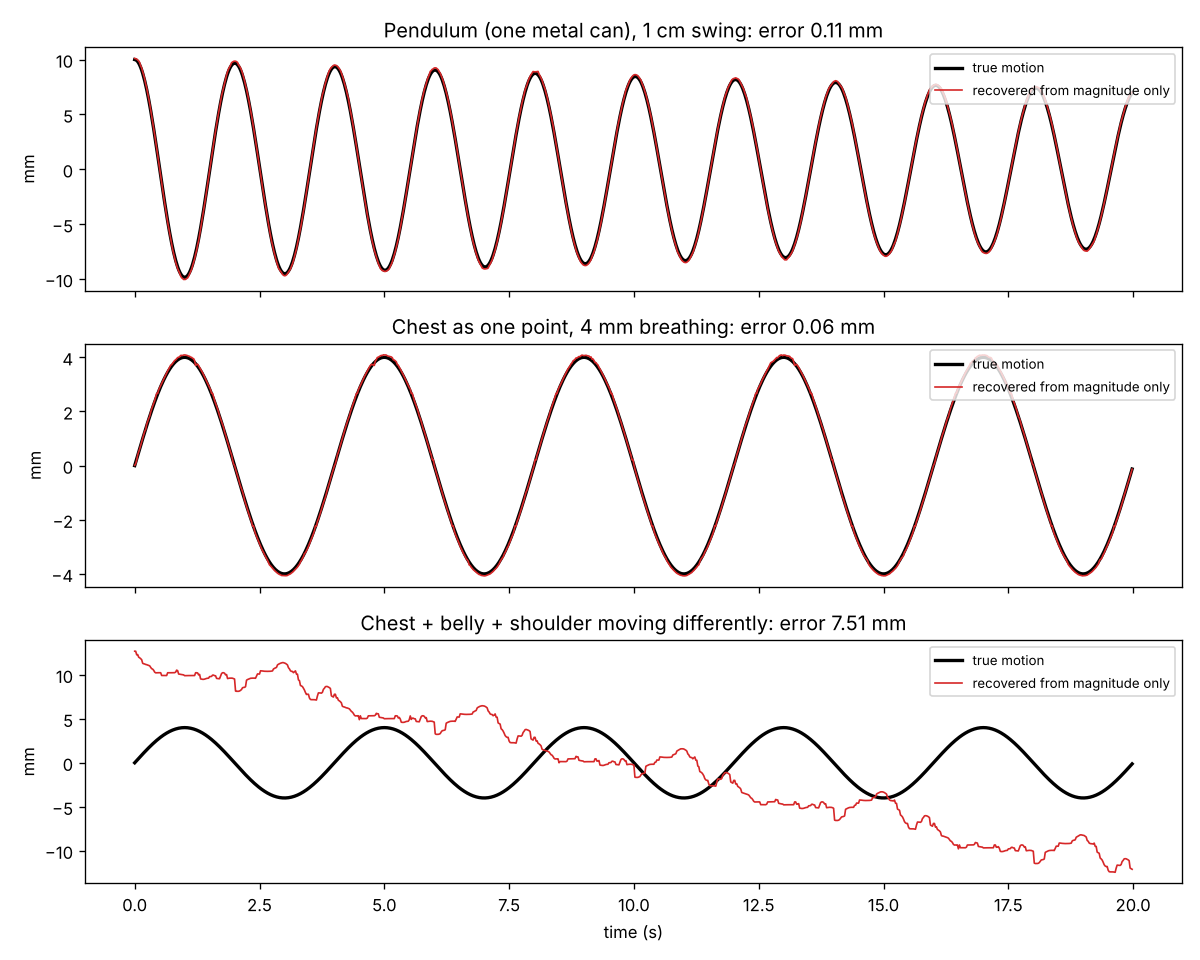
\includegraphics[width=0.85\linewidth]{figs/fig_phase_retrieval_sim.png}
\caption{Simulation: true motion and motion recovered from magnitude-only range profiles (sign and offset aligned). A single reflector is recovered to a tenth of a millimetre; a body made of several parts moving differently is not.}
\label{fig:prsim}
\end{figure}

\paragraph{Real data.} On the 50-frames-per-second breathing recording the model fits the data less well (coefficient of determination 0.85 to 0.91, against 0.99 in the single-reflector simulation and 0.81 in the three-part one), and the recovered displacement changes with the choice of range bins and contains jumps that a chest cannot make. I do not consider it a measurement. A first test with a known motion, a metal pot pulled \SI{5}{cm} towards the radar with a strip of tape, also failed: the method found 7 to \SI{13}{mm} depending on the bins. The recording suggests why, although the causes cannot be separated with one recording. My arm was moving in the field of view, the tape made the pot move in jerks (so the phase jumped by more than half a turn between frames and turns were lost), and \SI{5}{cm} is almost half a range bin, which breaks the assumption that the echo amplitudes stay constant.

\paragraph{What this shows.} The approach works in simulation for a single dominant reflector. The real recordings at 50 frames per second do show breathing-related changes of the magnitude, but recovering the displacement from them has not worked so far. One likely reason is that several body parts move differently, which the simulation reproduces. Two other candidates cannot be ruled out: the antenna combination inside the firmware, which I could not verify, and a body echo that changes amplitude as well as phase. I have not been able to separate these causes. The next step is a test that matches the conditions under which it works in simulation: a small metal reflector on a pendulum, swinging by a few millimetres with nobody in the field of view, whose true motion follows from the length of the string. If that works, a small reflector taped to the chest would turn the body into something much closer to a single scatterer.

%=====================================================================
\section{Follow-up C: can the radar see a damaged propeller?}\label{sec:prop}
%=====================================================================

If the drone signature comes from the blades, damage to a blade should change it. This would make the radar useful not only for finding drones but for checking them. I cut one blade of one propeller step by step and recorded the drone, fixed in place \SI{0.5}{m} from the radar at full throttle, after each step (configuration as in the main experiment).

\begin{table}[h]
\centering\small
\caption{Propeller damage. ``High band'': mean level of the Doppler spectrum at $|v| > \SI{10}{m/s}$, in dB above the map median. *The first half-blade recording was taken while the cut propeller rubbed against the drone frame. Distances are nominal tape distances; the radar reports 0.59 and \SI{0.70}{m}.}
\label{tab:prop}
\begin{tabular}{@{}llccc@{}}
\toprule
Distance & Propeller & High band (dB) & Skirt (dB) & Note \\
\midrule
\SI{0.5}{m} & intact & 4.48 & 6.36 & \\
\SI{0.5}{m} & intact & 4.62 & 6.87 & repeat \\
\SI{0.5}{m} & 2\,mm cut from one blade tip & 4.41 & 6.74 & \\
\SI{0.5}{m} & 7\,mm cut & 4.87 & 7.09 & \\
\SI{0.5}{m} & half of one blade cut* & 2.11 & 3.88 & rubbing \\
\midrule
\SI{0.6}{m} & new propeller & 2.48 & 4.11 & last 6.5\,s \\
\SI{0.6}{m} & same, half of one blade cut & 1.73 & 3.75 & last 6.5\,s \\
\bottomrule
\end{tabular}
\end{table}

\begin{figure}[t]
\centering
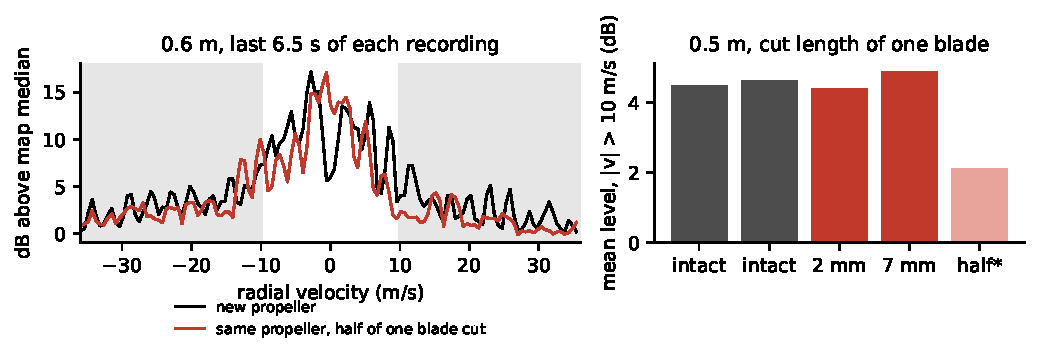
\includegraphics[width=0.95\linewidth]{figs/propeller.pdf}
\caption{Left: spectra of the controlled pair at \SI{0.6}{m}, before and after cutting half of one blade. Right: high-band level for each step at \SI{0.5}{m} (*rubbing against the frame).}
\label{fig:prop}
\end{figure}

Cuts of 2 and \SI{7}{mm} made no measurable difference: their high-band values lie within about \SI{0.3}{dB} of the intact recordings, comparable to the \SI{0.14}{dB} between the two intact ones, and they showed no consistent direction: the \SI{2}{mm} cut lay \SI{0.07}{dB} below the lower intact value, the \SI{7}{mm} cut \SI{0.25}{dB} above the higher one (Table~\ref{tab:prop}, Figure~\ref{fig:prop}). Cutting half of one blade produced a large drop in the high band, but that propeller was rubbing against the frame, which slows it down, and the battery was low by then; either could explain the drop. I therefore repeated the step in a controlled way: a new propeller recorded intact, then cut, back to back at the same place and battery level, using only the last 6.5 seconds of each recording, when the drone had settled. The high band fell from 2.48 to \SI{1.73}{dB}, a drop of \SI{0.75}{dB}, about three to five times the variation between and within intact recordings. The lower part of the spectrum fell as well, and by more: the mean level of the moving bins below \SI{10}{m/s} dropped from 10.2 to \SI{8.3}{dB}. The change is therefore not specific to the blade tips; an overall weaker echo, for example from a slower motor or a slightly different orientation, would explain it just as well.

This is a preliminary observation, not damage detection: with this chirp, cuts of 2 and \SI{7}{mm} showed no change, and cutting half of one blade was associated with a small drop of the whole moving spectrum, not only of the part that a shorter blade should affect. It rests on one controlled pair of recordings, and the propeller speed was not measured, so a change of motor speed caused by the imbalance cannot be excluded. Repeated measurements are needed before calling it a result. The main obstacles are clear. The damaged blade is one of eight blades in the same range bin, and the signature of imbalance, extra lines spaced by the rotation rate of a few hundred hertz, would lie only one to two of our \SI{230}{Hz} Doppler bins apart, and these are further smeared by the four rotors and by aliasing. A useful propeller check would need a longer coherent dwell (more chirps per frame), one rotor measured at a time, and an independent measurement of the rotation rate, for example from sound.

%=====================================================================
\section{Limitations}\label{sec:limits}
%=====================================================================

\begin{itemize}
\item \textbf{Range.} With the global detection gate, a tethered palm-sized drone was detected at \SI{1.2}{m} and not at \SI{1.9}{m}; the radar equation puts this limit at about 1.6 to \SI{1.7}{m}. A per-cell detector would probably reach further (Section~\ref{sec:det}), but this was not tested. This is a property of a tiny target and a low-power evaluation board, not a counter-drone system.
\item \textbf{One small independent test.} The cross-validated accuracies come from the data the settings were tuned on. The frozen test (Section~\ref{sec:test}) adds 20 new recordings (plus one at a lower radar height) and a second room, but with the same drone, fan and person, and only a few recordings per condition.
\item \textbf{One drone, one person, one fan.} The training data come from one room, one toy drone and me; the test added a second room but not another drone, person or fan. The classifier has never seen birds or outdoor clutter.
\item \textbf{One target at a time.} The classifier describes only the range row with the most moving energy. With a person and a fan or drone moving at the same time it mostly answers ``unsure'' (Section~\ref{sec:test}).
\item \textbf{Small data set.} 28 labelled recordings, about 1000 one-second windows. Overlapping windows are not independent, and the fold-to-fold spread (65 to 99\,\%) shows how much the result depends on which recordings are tested.
\item \textbf{Mostly tethered, not flying.} The training data contain one free flight, which was recognised in only 10\,\% of windows. Two short free flights in the test, close to the radar, were recognised in 97 and 98\,\% of frames; that is encouraging but too little to call free flight solved.
\item \textbf{No ground truth for propeller speed} and only approximate distances for the tethered drone.
\item \textbf{The demo firmware.} Only processed outputs were recorded: magnitude-only range-Doppler maps and range profiles, no raw samples and no phase (the demo can also send complex zero-Doppler data for its angle heatmap, which was switched off here), and an antenna combination I could not verify. This limits Sections~\ref{sec:still} to~\ref{sec:prop} most.
\end{itemize}

%=====================================================================
\section{Next steps}\label{sec:next}
%=====================================================================

\begin{itemize}
\item \textbf{Range:} replace the global gate by a per-cell CFAR detector with about one second of averaging, and test it on recordings at 2 to \SI{3}{m}; use all three transmitters for more gain at the price of $\vmax$.
\item \textbf{Scale:} derive the factor between map units and true dB (empirically 1.65 to 1.9) from the firmware source, and measure the board's EIRP with a reference reflector of known RCS (a corner reflector), which would turn the RCS estimate into a calibrated measurement.
\item \textbf{Several targets:} classify every moving range cell separately instead of only the strongest, so that a person next to a drone no longer turns the answer into ``unsure''.
\item \textbf{More varied data:} another drone, other people and fans, fans seen from different heights, longer free flights, and outdoor scenes.
\item \textbf{Rotation rate:} record the motor sound with a phone during each run and compare its fundamental frequency with the line spacing in the radar spectrum.
\item \textbf{Phase retrieval:} validate on a pendulum with a small metal reflector, then with a reflector on the chest; for ground truth, raw I/Q data from TI's capture board (DCA1000) would allow running the method on magnitudes while knowing the true phase.
\item \textbf{Propeller check:} longer dwell for finer Doppler resolution, a single rotor at a time, and repeated measurements per damage level.
\end{itemize}

%=====================================================================
\section{Conclusion}
%=====================================================================

A spinning propeller spreads its echo over the whole velocity axis of a 60\,GHz radar, and a handful of physically motivated features describing that spread were enough, in this data set, to tell a tethered toy drone apart from a person and a fan: once something was detected, 90.7\,\% of one-second windows of unseen recordings were classified correctly (79\,\% of drone windows), and counting every window, a drone tethered within about \SI{1.2}{m} was recognised 94\,\% of the time. A flying drone was recognised much less often. With the simple global gate the tethered drone was missed at \SI{1.9}{m}, as the radar equation predicts for that gate; in its own range cell, however, it stood clearly above the noise, so a per-cell detector should reach further. Once the board's map scale was corrected by an empirical factor of about two, the propeller echo fell with distance roughly as the radar equation predicts, and a model-dependent estimate of the propellers' radar cross section, not calibrated against a reference reflector, is of the order of \SI{1}{cm^2} (0.4 to \SI{1.7}{cm^2}). After smoothing, no person, fan or empty-room recording in the data set produced a drone label, at the cost of ``unsure'' labels and a slightly later decision. A frozen test on 20 new recordings, partly in a room the system had never seen, kept these properties within its limits: no false drone in any of its ten empty-room, person or fan recordings (correlated frames, so not a general false-alarm rate), and 98\,\% correct frames in five of the seven drone recordings, including two short free flights (82\,\% in a sixth, in which the drone fell off its pole). It also showed where the method stops: the drone at \SI{1.64}{m} was missed, a fan seen with the radar \SI{18}{cm} lower was never recognised, and two moving targets at once mostly gave ``unsure''. Other rooms, drones, people and geometries remain untested. Switching off static-clutter removal made a motionless person visible and, at 50 frames per second, a held breath. The phase retrieval method of my thesis recovered the motion of a single reflector to a tenth of a millimetre in simulation but has not worked on real data so far. A large cut in one blade was associated with a small spectral change in one controlled comparison. The most useful lesson of the project was that most wrong labels had a cause that could be found in the data, and that looking for it was usually more informative than the accuracy figure.

\paragraph{Tools.} TI mmWave SDK 3.x out-of-box demo firmware on the radar; Python with NumPy, SciPy, scikit-learn and Matplotlib on the laptop; \LaTeX\ for this report. I used an AI coding assistant (Claude) to help write the software.

\begin{thebibliography}{9}\small
\bibitem{richards} M.~A. Richards, \emph{Fundamentals of Radar Signal Processing}, 2nd ed. New York: McGraw-Hill, 2014.
\bibitem{chen} V.~C. Chen, \emph{The Micro-Doppler Effect in Radar}, 2nd ed. Boston: Artech House, 2019.
\bibitem{ti-ds} Texas Instruments, \emph{IWR6843AOP Single-Chip 60- to 64-GHz mmWave Sensor Antennas-On-Package (AOP)}, datasheet. \url{https://www.ti.com/lit/ds/symlink/iwr6843aop.pdf}
\bibitem{ti-uart} Texas Instruments, \emph{Understanding UART Data Output Format}, Radar Toolbox 3.30 documentation. \url{https://dev.ti.com/tirex/explore/content/radar_toolbox_3_30_00_06/software_docs/Understanding_UART_Data_Output_Format.html}
\end{thebibliography}

\appendix
%=====================================================================
\section{Recordings}\label{app:data}
%=====================================================================

\begin{table}[H]
\centering\scriptsize
\caption{Labelled recordings used for classification. Range: median target range found by the software (for empty rooms, the noise peak). Det.: share of one-second windows above the detection gate. SNR, skirt, occupancy: medians over frames. Replay: share of frames with the correct label in the leave-one-recording-out replay with smoothing.}
\label{tab:data}
\begin{tabular}{@{}lllrrrrrr@{}}
\toprule
Recording & Class & Description & Range (m) & Det. & SNR (dB) & Skirt (dB) & Occ. & Replay\\
\midrule
R01 & empty & nobody in view, fan off & 5.15 & 0\,\% & 3.8 & 1.31 & 0.00 & 100\,\% \\
R02 & empty & repeat & 5.33 & 0\,\% & 3.8 & 1.25 & 0.00 & 100\,\% \\
R10 & empty & third empty-room recording & 4.57 & 0\,\% & 3.7 & 1.29 & 0.00 & 100\,\% \\
R27 & empty & nobody in the room & 4.22 & 0\,\% & 3.7 & 1.32 & 0.00 & 100\,\% \\
R28 & empty & nobody in the room & 4.16 & 0\,\% & 3.7 & 1.35 & 0.00 & 100\,\% \\
R03 & fan & 2 m, facing, setting 1 & 2.23 & 100\,\% & 17.1 & 0.99 & 0.10 & 42\,\% \\
R04 & fan & 2 m, facing, setting 2 & 2.23 & 100\,\% & 16.7 & 0.98 & 0.12 & 97\,\% \\
R05 & fan & 2 m, facing, setting 3 & 2.23 & 100\,\% & 17.1 & 1.05 & 0.14 & 97\,\% \\
R06 & fan & 2 m, facing, setting 3, repeat & 2.23 & 100\,\% & 16.4 & 1.06 & 0.14 & 97\,\% \\
R15 & fan & 1 m, facing, setting 1 & 1.17 & 100\,\% & 22.6 & 0.95 & 0.15 & 97\,\% \\
R16 & fan & 1 m, facing, setting 3 & 1.17 & 100\,\% & 22.7 & 1.37 & 0.20 & 97\,\% \\
R23 & fan & 0.8 m, side-on, setting 1 & 0.94 & 100\,\% & 19.6 & 0.91 & 0.14 & 97\,\% \\
R24 & fan & 0.8 m, side-on, setting 3 & 0.94 & 100\,\% & 19.5 & 1.21 & 0.18 & 97\,\% \\
R07 & human & walking to and from, 2.5 m & 2.23 & 100\,\% & 21.6 & 1.05 & 0.02 & 98\,\% \\
R08 & human & walking to and from, 2.5 m & 2.34 & 100\,\% & 21.5 & 1.04 & 0.02 & 98\,\% \\
R09 & human & walking to and from, 2.5 m & 2.34 & 100\,\% & 21.7 & 1.05 & 0.02 & 98\,\% \\
R17 & human & waving arms, 2 m & 2.11 & 100\,\% & 16.6 & 1.04 & 0.02 & 91\,\% \\
R20 & human & walking close, 0.7 m & 0.94 & 100\,\% & 20.3 & 0.94 & 0.03 & 97\,\% \\
R21 & human & waving arms, 0.7 m & 0.94 & 100\,\% & 23.3 & 0.91 & 0.04 & 97\,\% \\
R22 & human & hand in front of radar, 0.5 m & 0.64 & 100\,\% & 25.1 & 0.84 & 0.06 & 44\,\% \\
R25 & human & standing almost still, 1.2 m & 1.35 & 100\,\% & 17.8 & 1.05 & 0.02 & 96\,\% \\
R26 & human & sitting, small hand moves, 1.2 m & 2.58 & 54\,\% & 8.1 & 1.19 & 0.01 & 18\,\% \\
R11 & drone & free flight, 0.5 to 1.5 m & 0.82 & 68\,\% & 12.7 & 1.13 & 0.03 & 5\,\% \\
R12 & drone & tethered, moving, 0.7 m & 0.59 & 100\,\% & 12.1 & 1.83 & 0.13 & 75\,\% \\
R13 & drone & tethered, 1.7 m & 1.87 & 0\,\% & 6.7 & 1.15 & 0.02 & 0\,\% \\
R14 & drone & tethered, 1 m & 1.17 & 100\,\% & 11.4 & 2.25 & 0.09 & 98\,\% \\
R18 & drone & tethered, 0.5 m & 0.59 & 100\,\% & 16.5 & 7.53 & 0.50 & 94\,\% \\
R19 & drone & tethered, 0.7 m, to the left & 0.94 & 100\,\% & 12.8 & 1.90 & 0.07 & 98\,\% \\
\bottomrule
\end{tabular}
\end{table}

Further recordings: four breathing recordings (4, 4, 20 and 50 frames per second; Section~\ref{sec:still}), one metal-pot recording at 50 frames per second (Section~\ref{sec:pr}), seven propeller recordings (Table~\ref{tab:prop}). Four recordings were discarded because the drone did not run properly or the propeller hit the frame; they are kept separately in the repository. The 20 test recordings, T03x and the four set-aside test recordings are listed in Table~\ref{tab:test} and Section~\ref{sec:test}.

%=====================================================================
\section{Configuration file}\label{app:cfg}
%=====================================================================

\begin{lstlisting}[language={},basicstyle=\ttfamily\scriptsize]
sensorStop
flushCfg
dfeDataOutputMode 1
channelCfg 15 1 0                         % 4 RX, 1 TX
adcCfg 2 1
adcbufCfg -1 0 1 1 1
profileCfg 0 60 10 6 24 0 0 100 1 64 5000 0 0 158
chirpCfg 0 0 0 0 0 0 0 1
frameCfg 0 0 128 0 250 1 0                % 128 chirps, 250 ms
lowPower 0 0
guiMonitor -1 1 1 0 0 1 1                 % points, range profile, RD map, stats
cfarCfg -1 0 2 8 4 3 0 15 1
cfarCfg -1 1 0 4 2 3 1 15 1
multiObjBeamForming -1 1 0.5
clutterRemoval -1 1                       % 0 in the breathing profiles
calibDcRangeSig -1 0 -5 8 256
extendedMaxVelocity -1 0
lvdsStreamCfg -1 0 0 0
compRangeBiasAndRxChanPhase 0.0 1 0 1 0 1 0 1 0 1 0 1 0 1 0 1 0 1 0 1 0 1 0 1 0
measureRangeBiasAndRxChanPhase 0 1.5 0.2
CQRxSatMonitor 0 3 5 31 0
CQSigImgMonitor 0 31 4
analogMonitor 0 0
aoaFovCfg -1 -90 90 -90 90
cfarFovCfg -1 0 0 7.4
cfarFovCfg -1 1 -35 35
calibData 0 0 0
sensorStart
\end{lstlisting}
The four-frames-per-second breathing profile changes only \texttt{clutterRemoval} (0). The 20 and 50 frames-per-second profiles also change \texttt{guiMonitor} (\texttt{-1 0 1 0 0 0 1}, range profile only) and \texttt{frameCfg} (50\,ms with 128 chirps, or 20\,ms with 32 chirps).

%=====================================================================
\section{Reproducing the results}\label{app:repro}
%=====================================================================

\begin{lstlisting}[language=bash]
python3 scripts/check_board.py                  # find ports, print chirp numbers
python3 scripts/record.py --label drone --distance 0.5 --seconds 20 --note "..."
python3 scripts/train.py data/*.npz             # grouped CV, saves the model
python3 scripts/live.py --model models/model.joblib
python3 scripts/live.py --model models/model.joblib --replay <file>.bin  # .bin not published
python3 report/compute_results.py               # Sections 6.2-6.5, Appendix A
python3 report/extra_stats.py                   # folds, bootstrap, end-to-end table
python3 report/analysis_rcs.py                  # Sections 7.1, 7.2
python3 report/analysis_det.py                  # Section 7.3
python3 report/analysis_avg.py                  # Section 7.3, averaging
python3 report/make_figures.py                  # figures of Sections 6 and 11
python3 report/make_figures2.py                 # figures of Section 7
python3 report/make_figure_test.py              # figure of Section 8
python3 report/make_figure_still.py             # first figure of Section 9
python3 scripts/eval_test.py data_test/*.npz    # frozen test: checks, then labels
python3 report/compute_test.py                  # numbers of Section 8
\end{lstlisting}
\texttt{check\_board.py}, \texttt{record.py} and \texttt{live.py} also run without the board: \texttt{-{}-sim drone} (or \texttt{human}, \texttt{fan}, \texttt{empty}) replaces the radar by the simulator. The frozen model was saved with scikit-learn 1.9.1; other versions may warn when loading it.

\noindent\textbf{Not produced by these scripts:} the live-session figure (Figure~\ref{fig:live}), whose labels were read by hand from a screen recording that is not published; the fan-speed figure and widths (Figure~\ref{fig:fanspeed}); the before-and-after numbers of Section~\ref{sec:wrong}, which describe earlier versions of the pipeline; and the remaining figures and numbers of Sections~\ref{sec:still} and~\ref{sec:pr} (breathing at 20 and 50 frames per second, phase retrieval), which come from earlier analysis scripts that are not included. The recordings behind them are included, and the phase retrieval method itself is in \texttt{mmwd/phase.py}.

\medskip\noindent\textbf{The smoothing rule of the live view} (\texttt{classify.py}):
\begin{lstlisting}
self.probs = (self.probs + [self.model.predict_proba(x)[0]])[-self.smooth:]
p = np.mean(self.probs, axis=0)
k = int(np.argmax(p))
need = self.drone_conf if self.model.classes_[k] == "drone" else self.min_conf
if len(self.probs) < min(3, self.smooth) or p[k] < need:
    return "unsure", float(p[k]), f
return self.model.classes_[k], float(p[k]), f
\end{lstlisting}

\end{document}
